
\chapter{模拟程序设计及算法实现}
\label{chap:Code}
随着加速器的流强越来越高,束流模拟代码在束流动力学研究中的作用也越来越重要,
尤其是在例如C-ADS,SNS,ESS等加速器中\cite{li2013physics,henderson2014spallation,eshraqi2016ess},
其非线性空间电荷效应占据主导地位。
一个拥有更强大的计算能力以及更高的精确度的程序,是我们研究强流束流动力学所必须的。

根据前一章中介绍的物理模型,在本章中我们对模拟程序的架构设计、代码实现、以及并行化优化策略进行介绍。
我们首先介绍P-TOPO程序的整体结构,之后分别介绍了PIC算法在GPU上和CPU集群上的的实现,和Symplectic在GPU上的实现。

\section{P-TOPO程序结构}
我们开发了一个新的粒子模拟程序,命名为Parallel-Trace of Particle Orbits (P-TOPO),致力于研究强流加速器中的空间电荷效应问题\cite{li2016nonlinear,li2014envelope,li16collective,li2015space}。
P-TOPO使用C++语言开发,并且使用OpenMP进行并行化,目标是在普通多核PC机上快速模拟粒子在加速器中的行为。
P-TOPO使用时间t,而不是使用位置z,作为基本的独立变量,这是研究粒子的空间电荷效应非常自然的选择。即时使用位置z作为基本变量,在求解空间电荷力的过程中,也需要将粒子坐标转换为同一时间t下的时空间坐标。
在P-TOPO中,产生外场的一些加速器元件,例如各种磁铁,螺线管,RFQ,的外场使用元件的解析模型得到;而对于另外一些元件,例如超导腔,我们首先读取场文件\cite{studio2008cst},然后采用二阶插值的方法获取粒子所受到的场的大小和方向。

对于束团内部的空间电荷效应,我们使用经典的PIC方法进行求解\cite{hockney1988computer}。PIC方法是研究空间电荷效应非常常用的的一种数值模拟算法\cite{PIC_birdsall2004plasma,PIC_luccio2002space}。PIC发展于上世纪七十年代,被广泛的应用于等离子体模拟和加速器设计。

P-TOPO的程序的结构如图\ref{fig:P_TOPO}所示,图中每一个条目为一个类:
\begin{itemize}
  \item 主类MAIN调用其他各个具体的类,比如从外部Lattice结构中获取外场,求解内部空间电荷力,以及根据粒子所受的场推动粒子的位置和动量。
  \item Lattice类根据外部输入文件,解析或者数值地构建加速器的结构,以及根据粒子坐标,给出粒子所受的外场力。
  \item Distribution类产生粒子的初始分布,目前可以产生 KV,Waterbag,Parabolic,和Gaussian四种粒子分布,如图\ref{fig:distribution}所示。
  \item Beam类统计粒子的信息,并且计算出如rms大小,发射度等束团参数,将其保存以供进一步分析和输出。
  \item Internal Field类通过PIC方法计算空间电荷效应,在PIC方法中,我们使用FFT 来求解Poisson方程。
  \item Leapfrog类和Runge-Kutta 4类都是继承Pusher类,是不同的推动粒子位置和动量的方法。
\end{itemize}

\begin{figure}[!htb]
    \centering
    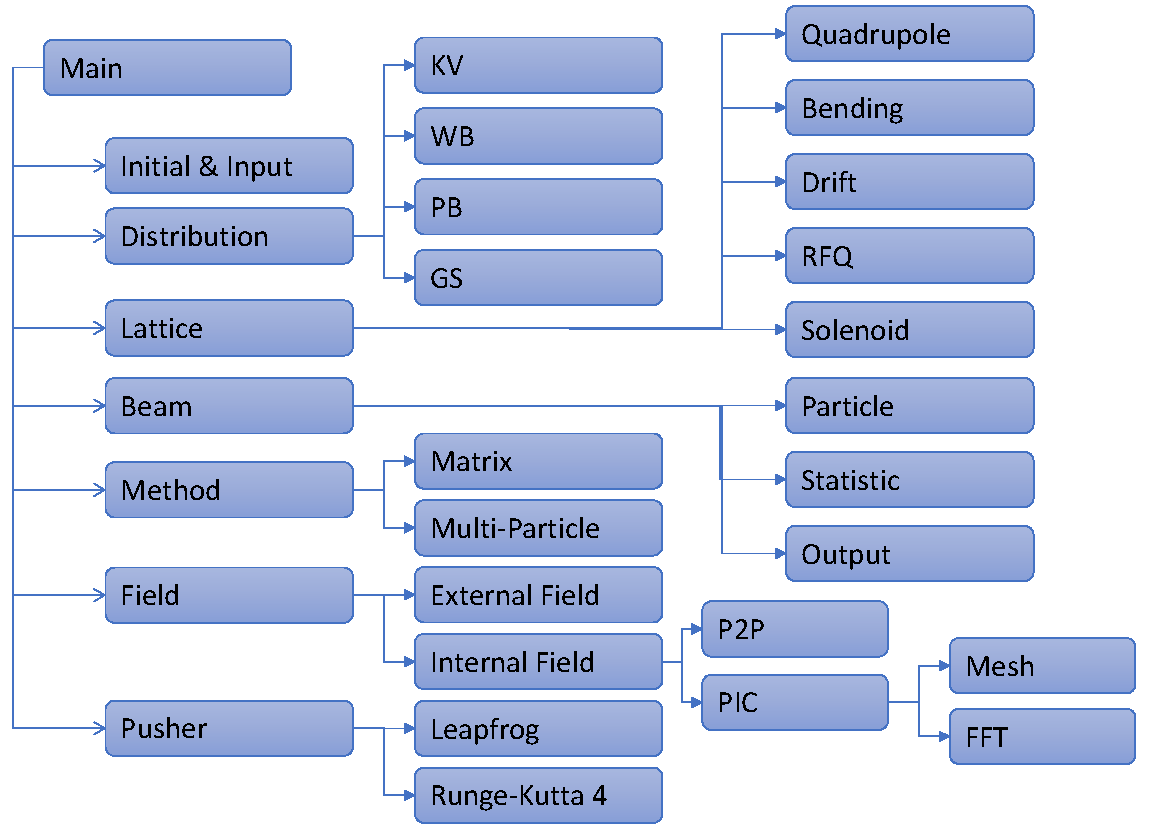
\includegraphics[width=0.8\textwidth]{Img/P_TOPO.pdf}
    \caption{P-TOPO程序结构}
    \label{fig:P_TOPO}
\end{figure}

\begin{figure}[!htb]
    \centering
    \begin{subfigure}[b]{0.48\textwidth}
        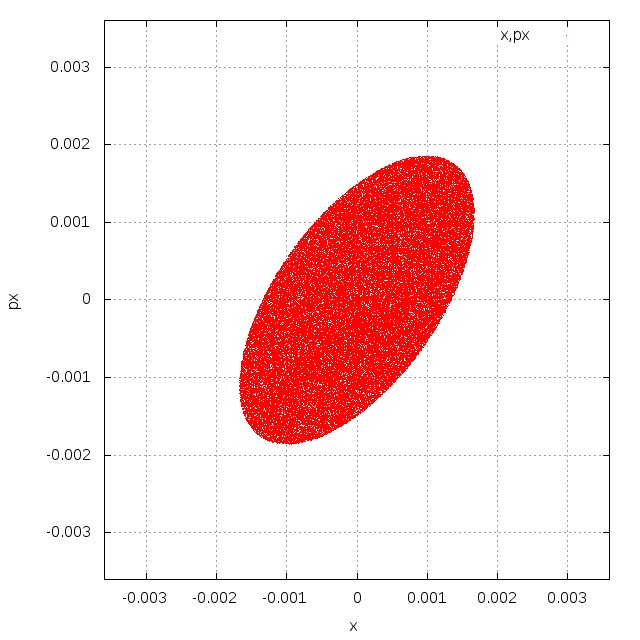
\includegraphics[width=\textwidth]{Img/KV_x_dx.jpg}
        \caption{KV}
    \end{subfigure}
    \begin{subfigure}[b]{0.48\textwidth}
        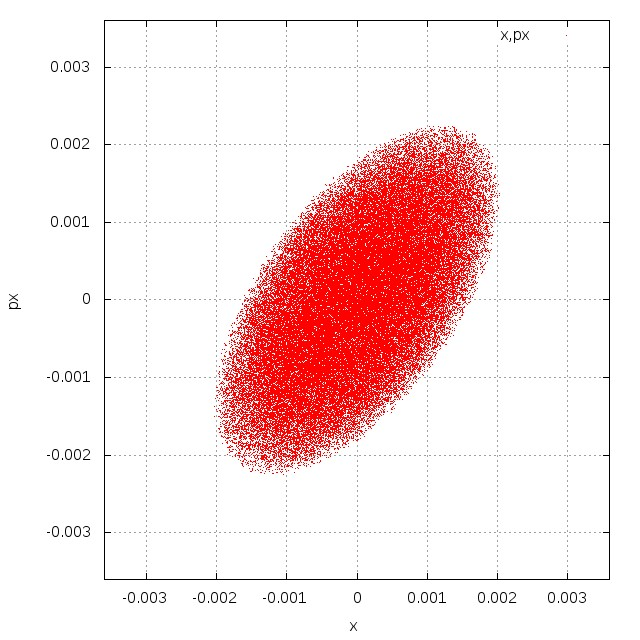
\includegraphics[width=\textwidth]{Img/WB_x_dx.jpg}
        \caption{Waterbag}
    \end{subfigure}
    \begin{subfigure}[b]{0.48\textwidth}
        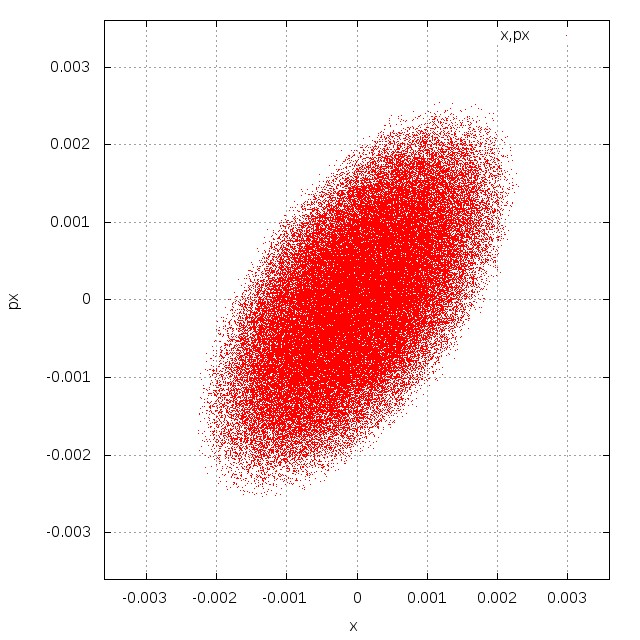
\includegraphics[width=\textwidth]{Img/PB_x_dx.jpg}
        \caption{Parabolic}
    \end{subfigure}
    \begin{subfigure}[b]{0.48\textwidth}
        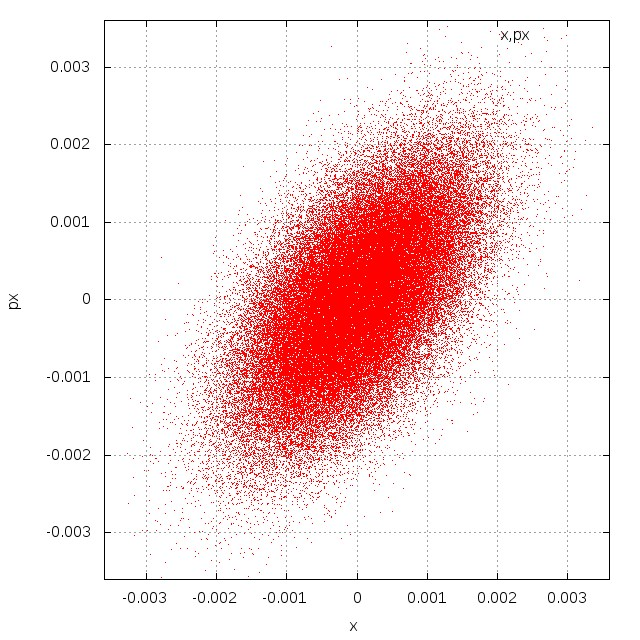
\includegraphics[width=\textwidth]{Img/GS_x_dx.jpg}
        \caption{Gaussian}
    \end{subfigure}
    \caption{同一均方根尺寸下的不同种类束团分布}\label{fig:distribution}
\end{figure}

程序主循环中的大部分都是并行化的,例如求解内场,推动粒子等。
最基本的,程序采用粒子并行策略,即每个线程处理不同的粒子。以粒子推动部分为例,如果粒子总数为160000,线程数为8,那么每个线程推动20000个粒子。
程序对可能发生线程冲突的部分,例如权重粒子,采用了其他的并行策略。除此之外,程序也使用了FFTW库的内部并行方法。


%程序也采用了一些其他的并行策略,以PIC求解Poisson方程为例,这部分需要4个独立的步骤来得到内部空间电荷场:
%\begin{enumerate}
%  \item 将粒子权重到网格,获得网格上的电荷密度;
%  \item 通过FFT求解网格上的Poisson方程,获得网格上的电势;
%  \item 对电势进行差分,获得网格上的电场;
%  \item 通过逆权重,得到粒子所在位置的电场。
%\end{enumerate}
%在第一步和第四步中,我们使用网格并行,即不同的线程处理不同的网格,这需要我们对粒子进行排序,以避免潜在的线程冲突。而在第二步和第三部中,主要的计算为傅里叶变换,程序使用了FFTW库的内部并行方法。

我们使用了一个4核的普通PC机进行性能测试,4线程运行的程序的速度是串行运行程序的3.6倍。关于程序的更大规模的并行问题,我们会在后文做进一步讨论。

\section{P-TOPO正确性校验}
\subsection{内场计算}
我们使用一个点电荷来测试PIC部分的正确性。使用的格点数目为 $128\times128\times64$。 横向边界为狄利克雷边界条件(第一类边界条件),纵向为周期性边界条件。 图\ref{fig:P_TOPO_verification1} 是P-TOPO 的结果与理论值的对比,其中左图为横向电势(X方向),右图为纵向电势(Z方向)。图中红色实线为程序通过PIC方法计算得到的电势场的大小,绿色虚线为理论值,可以看出,程序的结果与理论值非常吻合。

\begin{figure}[!htb]
    \centering
    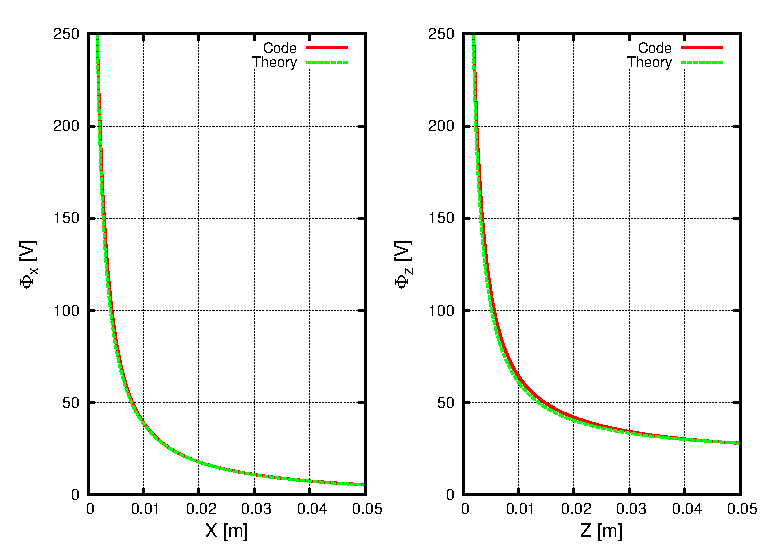
\includegraphics[width=0.8\textwidth]{Img/P_TOPO_verification1.eps}
    \caption{P-TOPO与理论值的点电荷电势对比}
    \label{fig:P_TOPO_verification1}
\end{figure}

\subsection{FD结构中与解析解的对比}
我们以束流在FD结构中束流的演化为例,来验证P-TOPO程序整体的正确性。连续束在周期聚焦结构中的束流包络方程可以表示为式\ref{eq:envelope}\cite{wangler1998particle,chen1994nonlinear}
\begin{equation}\label{eq:envelope}
  \frac{{{d}^{2}}R}{d{{z}^{2}}}+k_{0}^{2}R-\frac{{{\varepsilon }^{2}}}{{{R}^{3}}}-\frac{K}{R}=0
\end{equation}
其中$R$是束流横向均方根尺寸,$k_0$是聚焦强度,与外场力相关,$\varepsilon$为发射度,$K$是空间电荷力强度。束流的横向均方根尺寸与初始匹配和相移有关。
在这个验证中,计算空间电荷力的网格数目为64*64,我们使用10000个宏粒子在KV初始分布下,分别以0mA和15mA在周期性FD结构中前进,每个FD结构中推动400步。
图\ref{fig:P_TOPO_verification2}显示了由P-TOPO给出的束流均方根尺寸的演变和均方根包络方程的理论预期,其中图片下部浅蓝色线表示外部四级铁的聚焦强度,红色实线和绿色虚线分别为零流强下理论结果和P-TOPO程序计算结果,而蓝色实线和紫色虚线分别代表15mA流强下理论预期和P-TOPO计算结果。可以看出,无论是在零流强时还是15mA流强时,计算结果与理论值都保持高度一致,其中在15mA下束团演变的微小区别是因为包络方程计算中假定发射度为常数,而实际的PIC计算中发射度会发生变化。

\begin{figure}[!htb]
    \centering
    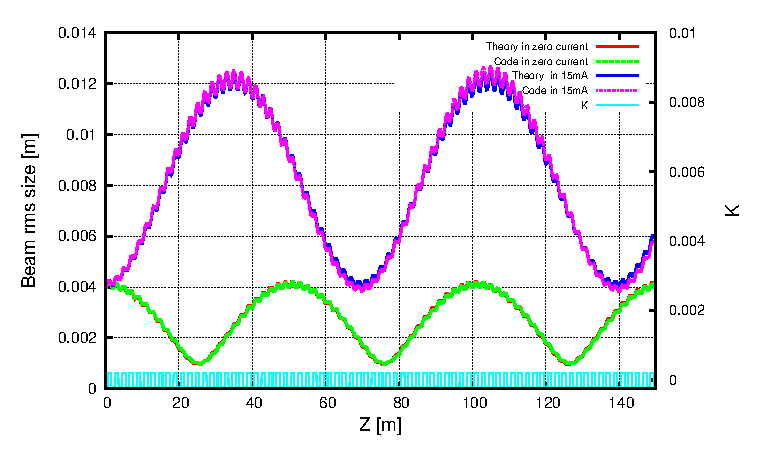
\includegraphics[width=0.8\textwidth]{Img/P_TOPO_verification2.eps}
    \caption{零流强和15mA时,P-TOPO结果与包络方程的对比}
    \label{fig:P_TOPO_verification2}
\end{figure}


%在本章中,首先,我们会介绍GPU程序的基本结构和并行策略。之后,我们做了一个GPU程序和CPU程序结果的对比,以验证程序的正确性。
%再后,我们展示了GPU程序的效率和在不同规模的问题下的加速比。
%最后,我们也实现了此程序在新的CPU架构,Knight Landing,上的并行化运行,并与GPU的运行效率进行了对比。

\section{PIC算法在GPU上的实现}
在\ref{section:PIC_algorithm}中我们介绍了基本的PIC算法。
PIC算法主要包括四部分:权重差值,解泊松方程,将场反权重到粒子,推动粒子。
在本章中,我们致力于在GPU上实现基于PIC算法的多粒子跟踪程序的并行化,提高程序的运行效率。
在GPU上实现PIC算法,主要难点在第一步权重差值上。第一步权重插值是将粒子逐个权重到网格上的过程,此步骤多线程并行运行时,会遇到不同线程相互竞争的问题(race condition),从而导致错误的结果。

线程竞争是指在程序中,协作的线程可能共享一些彼此都能读写的公用存储区,而竞争出现在当两个或多个线程同时访问同一内存地址,并且尝试写入数据的时候。由于线程调度器会以任意顺序运行多个线程,而我们无法得知线程尝试访问共享内存的顺序。因此,数据的最红结果会取决于线程调度器的算法,即多个线程“竞争”访问和改变数据。

图\ref{fig:PIC_weighting_threading}显示了PIC算法中权重差值部分的运算流程和多线程下可能会出现的竞争和冲突结果,其中蓝色点代表粒子,而绿色星状点代表与粒子相近的网格。使用多个线程运行权重插值时,通常使不同的线程处理不同的粒子。假设我们使用五个时钟锁步线程,如图\ref{fig:PIC_weighting_threading}中所示,线程A-E分别处理五个粒子。A,B,C三个线程并没有发生冲突,但是D线程和E线程会产生竞争,造成错误的运算结果。在第一个时钟周期内,线程D和E分别从同一内存地址M,读取格点原本的电荷量V;在第二个时钟周期,线程D读取粒子D的电荷并计算相应应该加到格点的电荷V+D,而线程E读取粒子E并计算得到V+E;在第三个时钟周期,线程D将V+D写入内存地址M,同时线程E将V+E写入同一内存地址M。但是两个写入都是错误,正确的结果应该是V+D+E。

\begin{figure}[!htb]
  \centering
  \begin{tabular}{|l|l|}
    \multicolumn{2}{c}{
    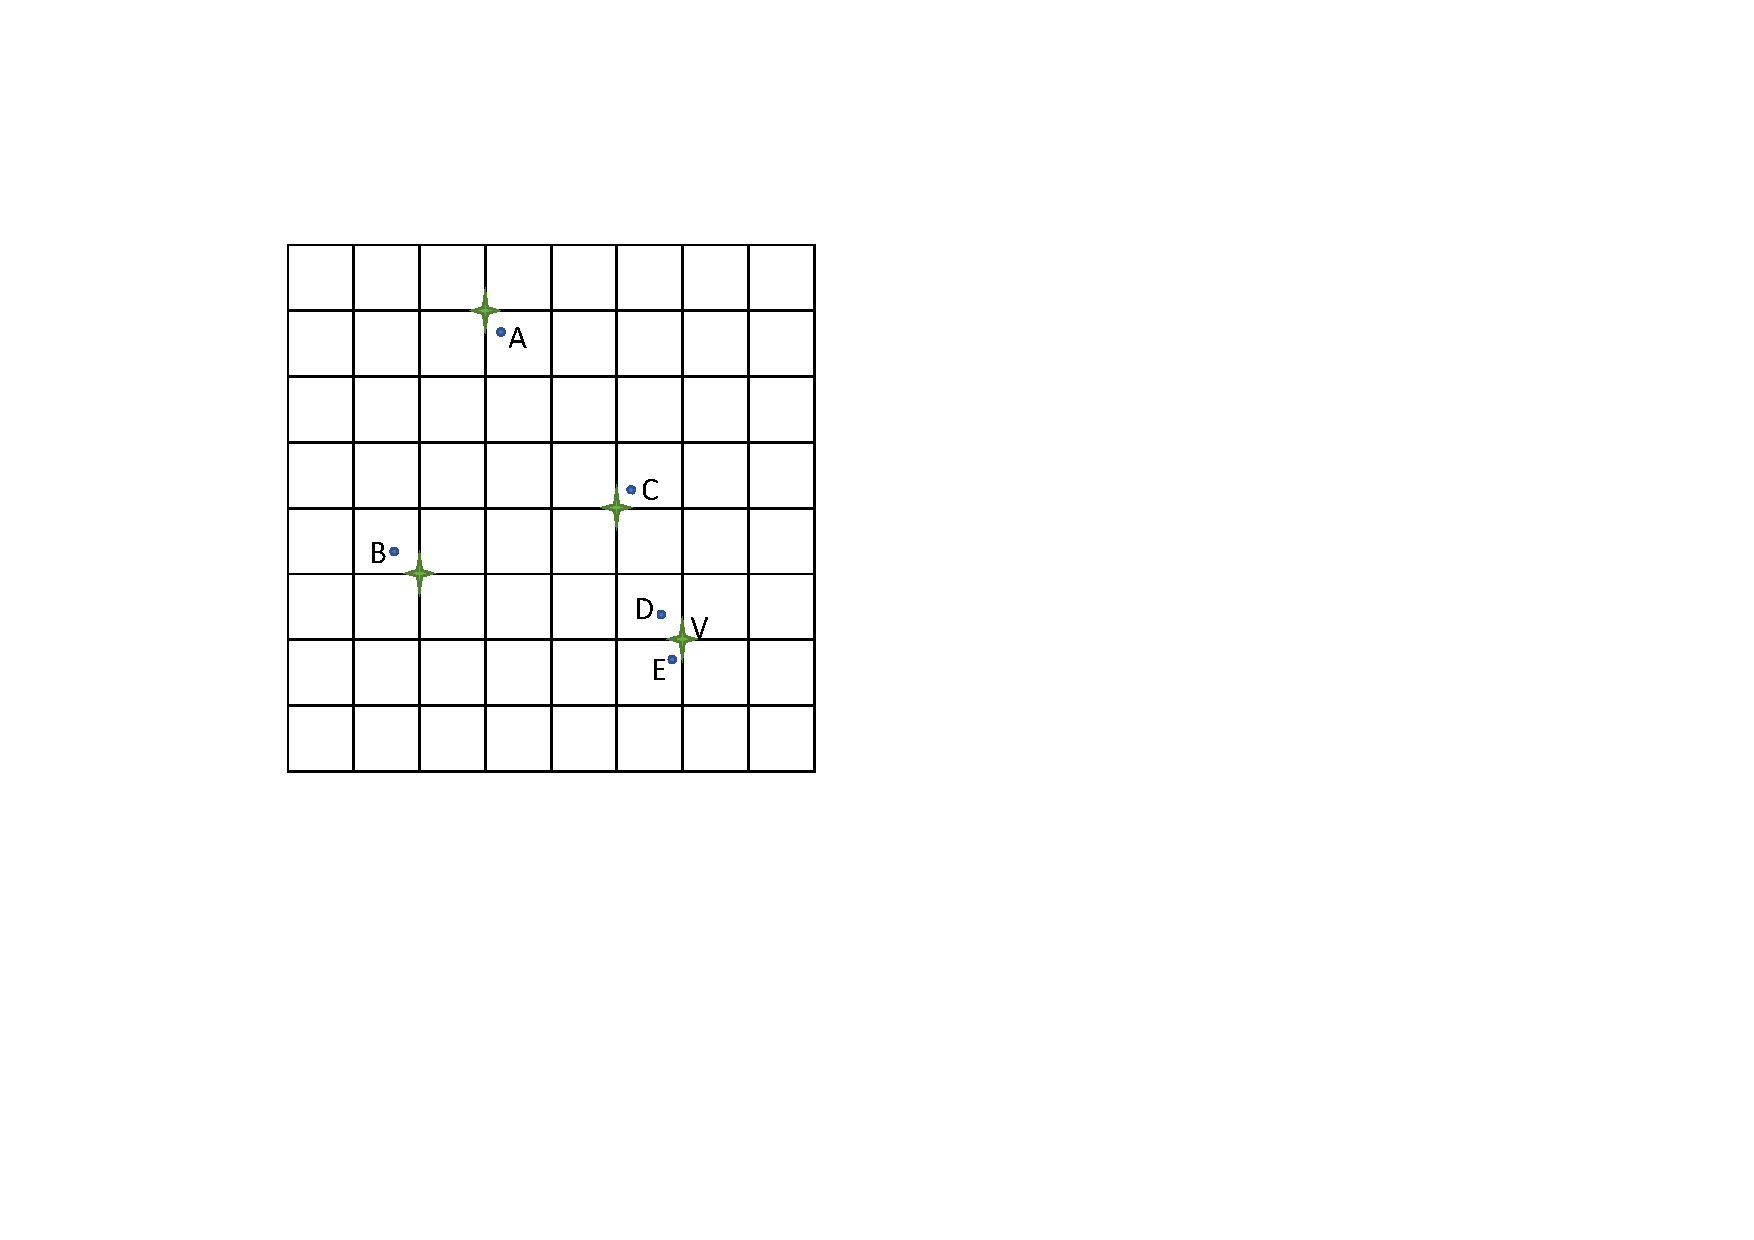
\includegraphics[width=0.65\textwidth]{Img/3PIC_weighting.pdf}} \\
  \end{tabular}
  \begin{tabular}{|l|l|}
    \hline
    Thread D & Thread E  \\
    \hline
    1D: Read variable V     & 1E: Read variable V     \\
    2D: Add D to variable V & 2E: Add E to variable V \\
    3D: Write back (V+D)    & 3E: Write back (V+E)    \\
    \hline
    \multicolumn{2}{c}{But it should be V + D + E!}
  \end{tabular}
  \caption{权重差值中的线程冲突}
  \label{fig:PIC_weighting_threading}
\end{figure}

为了避免线程之间的竞争和冲突,我们采取先将网格分块,再随后将网格上的电荷合并的做法。如图\ref{fig:PIC_tile}所示,绿色部分为一个区块,而一个线程单独处理一个区块。想要分块处理,粒子必须是有序的,这样才能使相应的线程找到所对应区域的粒子。所以在插值权重之前,我们需要对粒子进行排序(reorder)。假设区块数目为N,我们需要声明N个数组,以分别对应N个区块中的粒子。在程序初始阶段,我们将粒子数据拷贝到不同的区块数组中,并且在随后的每一步中,粒子可能改变位置,所以我们要对粒子重新排序,以确保粒子处于所对应的区块数组。用这种方法,每一个线程能够单独处理自己所分配的区块,从而避免了线程之间的竞争和冲突。加入了排序之后的PIC算法流程如图\ref{fig:PIC_flow_reorder}所示,其中,标识为红色部分为粒子排序,是PIC算法在GPU上并行运行所必须的前置步骤;而黄色部分的GPU算法和普通CPU算法有较大区别,我们在下面,对流程图种的黄色部分,即GPU上的PIC算法中的粒子排序,权重插值,解泊松方程,以及粒子推动做进一步讨论。

\begin{figure}[!htb]
    \centering
    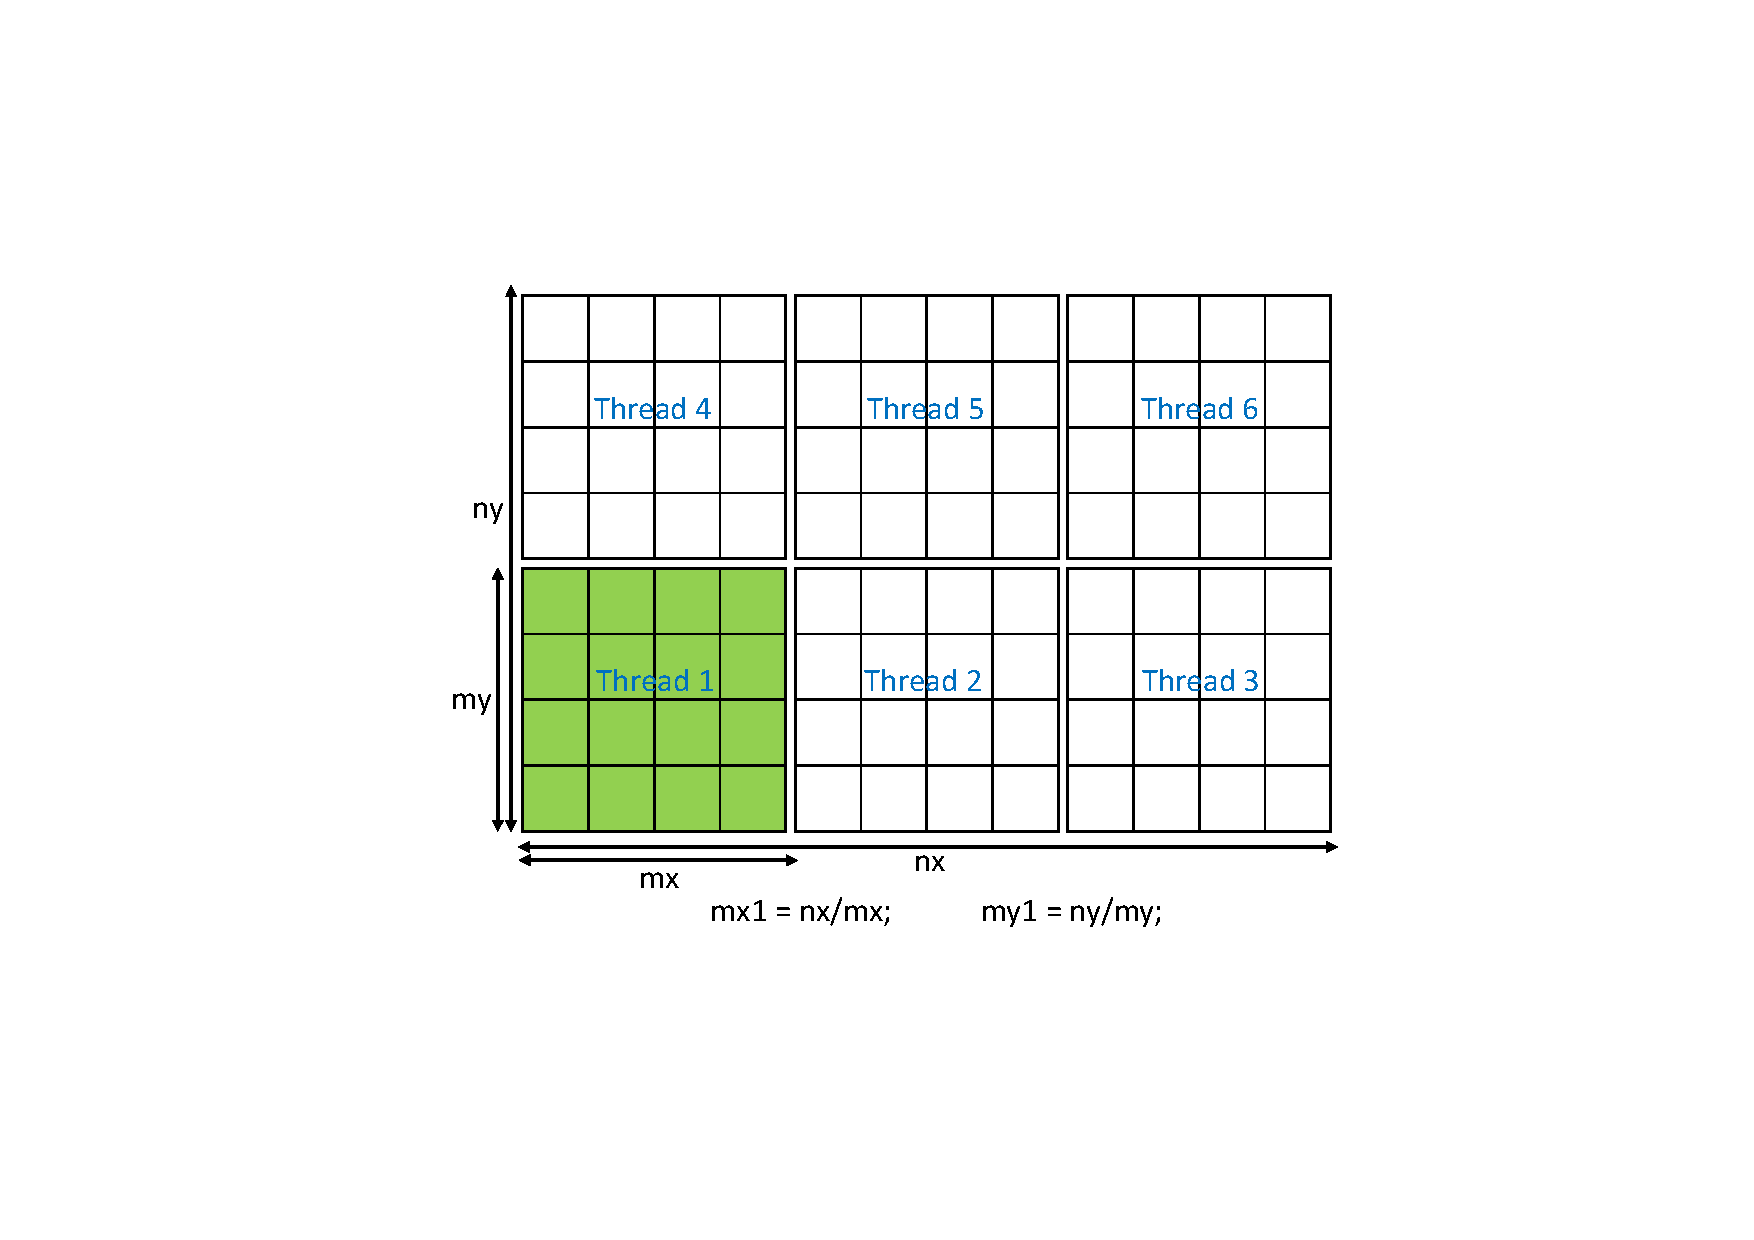
\includegraphics[width=0.85\textwidth]{Img/3PIC_tile.pdf}
    \caption{网格分块示意图}
    \label{fig:PIC_tile}
\end{figure}

\begin{figure}[!htb]
    \centering
    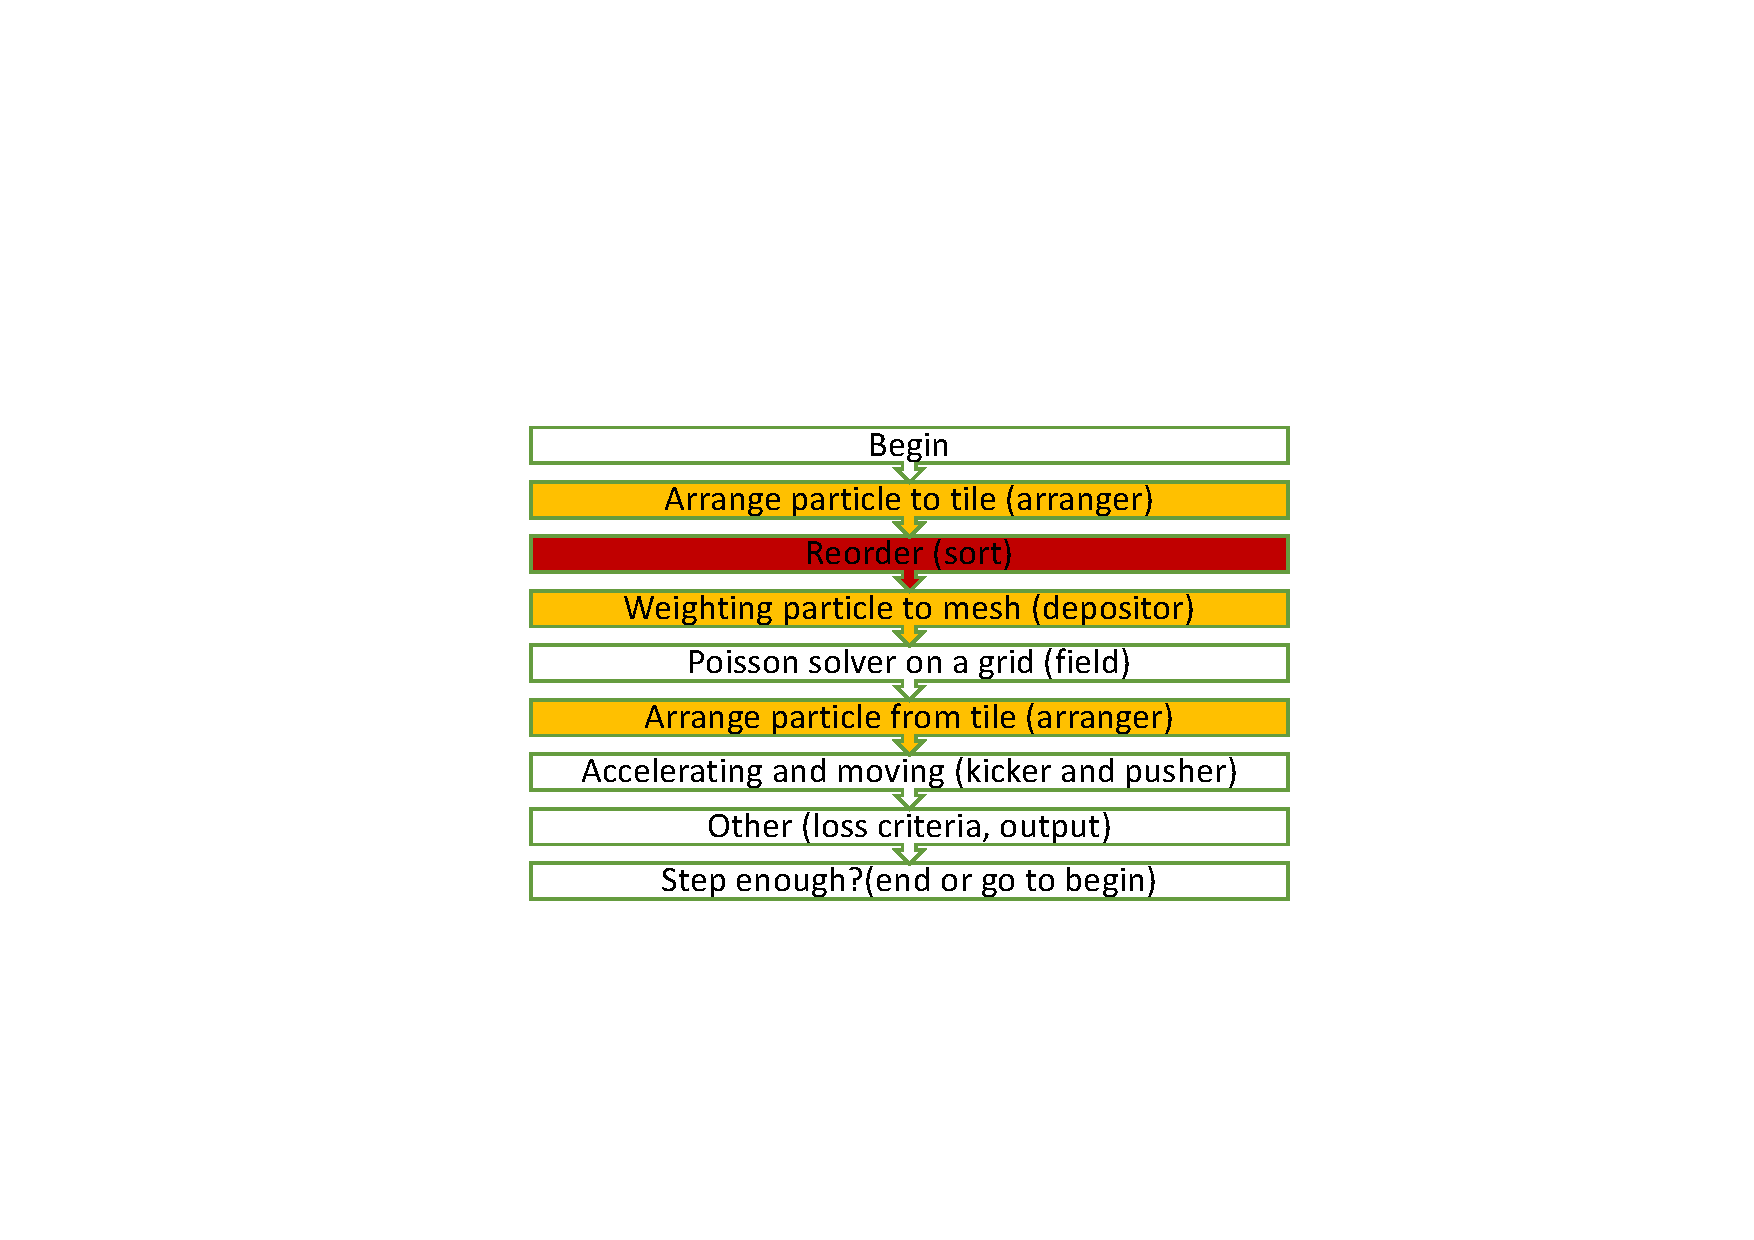
\includegraphics[width=0.75\textwidth]{Img/3PIC_flow_reorder.pdf}
    \caption{GPU上的PIC算法分段流程}
    \label{fig:PIC_flow_reorder}
\end{figure}



\subsection{粒子排序}
\label{section:PIC_GPU_reorder}
如上所述,GPU上PIC算法中,我们必须要将粒子在每一步进行重新排序,以避免线程竞争。排序在GPU中的实现并不直接,因为其高度不规则的并且难以并行执行。在这里,我们使用临时缓冲区作为中继,以实现粒子排序算法在GPU上的并行运行。
我们将整个网格划分为不同的区块,使每个线程只需处理对应的区块即可。例如,在一个网格数为$64 \times 64 \times 64$的模拟中,我们将其分割成大小为4*4*4的区块,总共$16 \times 16 \times 16$=4096个区块,这样我们可以避免线程的竞争。

在程序初始化的时候,我们首先需要为每一个区块声明数组并为其分配内存空间,如以下代码所示。
其中,我们根据实际使用的GPU的可用内存大小来确定每个区块的最大粒子数目。如果某一区块的粒子数目超过了最大粒子数,程序会报错并停止。在这种情况下,使用更少的粒子数目或者使用内存更大的显卡可以解决问题。
因为在实际模拟中,每个区块的粒子数一般并不相同,使用内存预分配会导致浪费很多内存空间。但是不同于CPU内存,在GPU上分配内存耗时很长,所以无法在每一步计算中根据实际情况来进行内存的分配,只能采用预分配的方法,以提高程序运行效率。
\begin{lstlisting}
  const int lth =BLOCKSIZE;
  const int dim =_dimension;
  int mth       = (mx1*my1*mz1-1)/lth+1;    //number of tiles

  double *ptc;       //tiled particle
  int    *kpic;      //number of particles in each tile
  int    *nhole;     //number of hole left
  int    *ncl;       //ndirec[k*26 + i]: number of particle going
                     //to destination i[0-26) from tile k
  double *pbuff;     //buffer for transfer particles

  //get the maximum number of particle according to the GPU memory size
  size_t freeMem,totalMem;
  cuda_SafeCall(cudaMemGetInfo(&freeMem,&totalMem));
  int npm = freeMem / 2 / sizeof(double) / dim / (mx1*my1*mz1);
  if(npm>numberOfParticle) npm = numberOfParticle;
  int MaxPtcTransf = npm / 2;


  //allocate memory for particle array
  size_t ptc_mem_size = sizeof(double)*lth*dim*npm*mth;
  cuda_SafeCall(cudaMalloc((void**) &ptc,     ptc_mem_size));

  //allocate memory for particle counting array
  size_t kpic_mem_size=sizeof(int)*mx1*my1*mz1;
  cuda_SafeCall(cudaMalloc((void**) &kpic,    kpic_mem_size));

  //allocate memory for holes at tiles array
  size_t nhole_mem_size = sizeof(double)*lth*2*(MaxPtcTransf+1)*mth;
  cuda_SafeCall((cudaMalloc((void**) &nhole,  nhole_mem_size));

  //allocate memory for particle buffer array
  size_t pbuff_mem_size = sizeof(double)*lth*dim*MaxPtcTransf*mth;
  cuda_SafeCall((cudaMalloc((void**) &pbuff,  pbuff_mem_size));

  //allocate memory for transferred particle counting array
  size_t ndirec_mem_size = sizeof(int)*mx1*my1*mz1*(3*3*3-1);
  cuda_SafeCall((cudaMalloc((void**) &ndirec, ndirec_mem_size));
\end{lstlisting}

在之后的每一步计算中,在空间电荷效应之前,我们都需要根据粒子空间位置对粒子进行排序,排序流程如图\ref{fig:PIC_reorder}所示:
\begin{figure}[!htb]
    \centering
    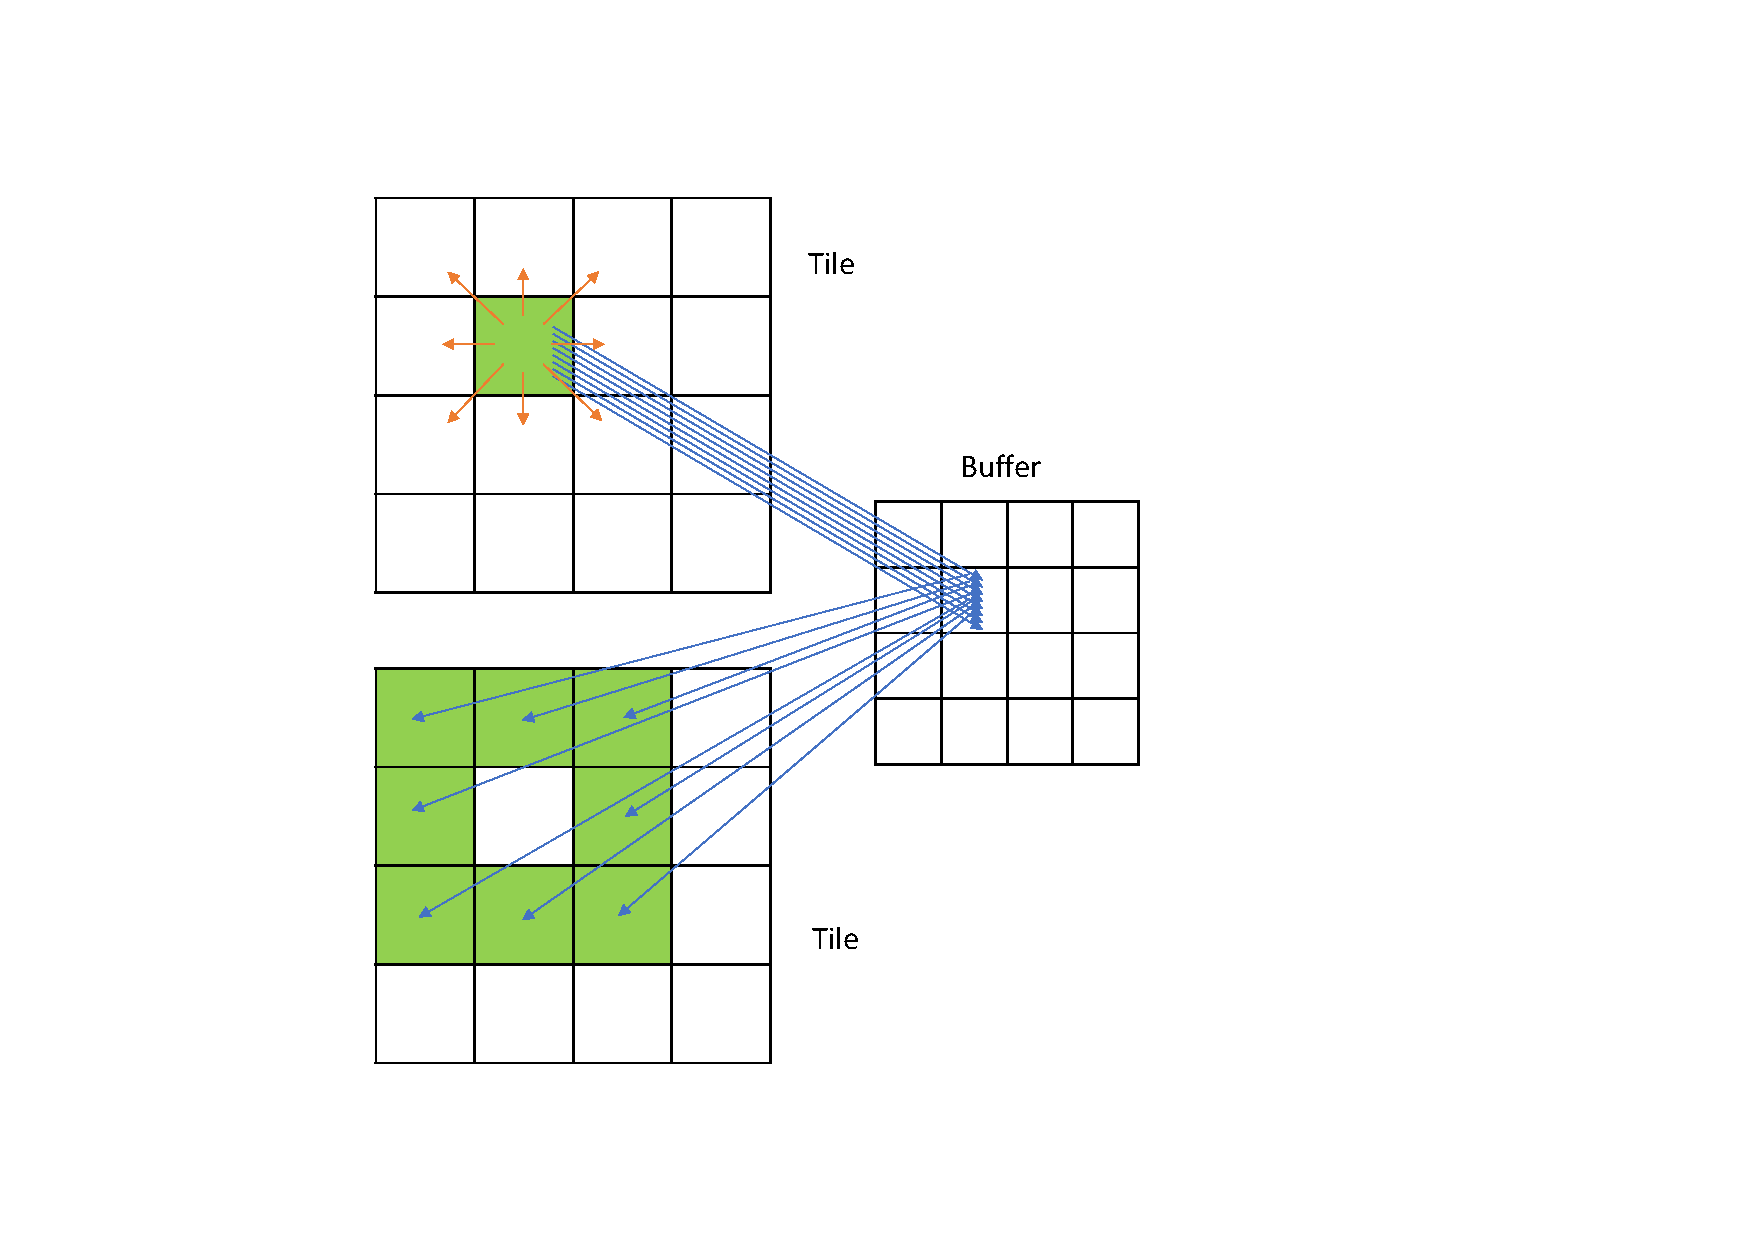
\includegraphics[width=0.75\textwidth]{Img/3PIC_reorder.pdf}
    \caption{粒子排序示意图}
    \label{fig:PIC_reorder}
\end{figure}

首先,每个线程统计对应区块中将要离开当前区块的粒子信息,并使用数组\verb"nhole"和\verb"ndirec"记录粒子的序号和每个方向的数目。如图\ref{fig:PIC_reorder}中黄色箭头所示。如上面代码所示,我们使用最大粒子数目的一半作为最大穿越数目,而\verb"nhole"已经根据最大穿越数目进行了内存预分配,同样的,如果离开当前区块的粒子数目超过了最大穿越数目,程序会报错停止,这时候需要使用更少的粒子数目或者更大的GPU内存。

之后,我们将离开当前区块的粒子信息拷贝到一个缓冲区\verb"pbuff"。作为全局内存,\verb"pbuff"同样根据最大穿越数目进行了内存预分配。\verb"ndirec"包括了每个方向上的粒子数目,对\verb"ndirec"进行迭代求和(running sum),我们可以得到每个方向上的内存初始位置,以便于将前往某个方向的粒子在\verb"pbuff"中连续排布。

最后,对于每个区块,经过第一步的统计,我们可以知道会有多少粒子进入,以及它们在\verb"pbuff"中的位置。在将粒子信息从\verb"pbuff"拷贝到当前区块\verb"ptc"的过程中,我们先填满因为粒子离开造成的空洞。如果如果进入的粒子数目大于空洞数目,即在所有空洞都被填满后,仍有粒子进入,我们将其写入在当前区块\verb"ptc"的最后;但如果进入的粒子数目小于空洞数目,即写入所有进入粒子后仍有空洞存在,则从本区块粒子数组\verb"ptc"尾部开始,依次移动粒子数据到空洞处。通过这种方式,粒子信息在内存中的连续性得到了保证。

我们对上述步骤做了一个简要总结,通过这些排序流程,使每个线程仅处理对应的区块,来确保不会出现线程竞争。

\begin{itemize}
  \item 首先,对本区块内的粒子进行遍历,将因为位置改变而不再属于本区块的粒子序号,以及其离开的方向记录下来,写入\verb"nhole" 和\verb"ndirec"。
  \item 其次,根据其序号和方向,将离开的粒子拷贝进入全局缓存区\verb"pbuff"。
  \item 最后,再根据相邻区块离开粒子的序号和方向,确定将要进入本区块的粒子,将缓存区内的数据拷贝到本区块。
\end{itemize}


\subsection{权重插值}
\label{section:PIC_GPU_depositor}
通过以上粒子重排,我们使得每一个区块的粒子相对独立,这样,我们可以使每个线程处理一个区块,从而避免了线程冲突的情况。
一个直接的权重插值流程如图所示\ref{fig:PIC_combine}:
\begin{itemize}
  \item 首先,每个线程将自己所处理的粒子权重到一个小网格上,得到本地的网格密度分布。
  \item 然后,我们将所有本地的密度分布结合到一起,得到全局密度分布。
\end{itemize}
\begin{figure}[!htb]
    \centering
    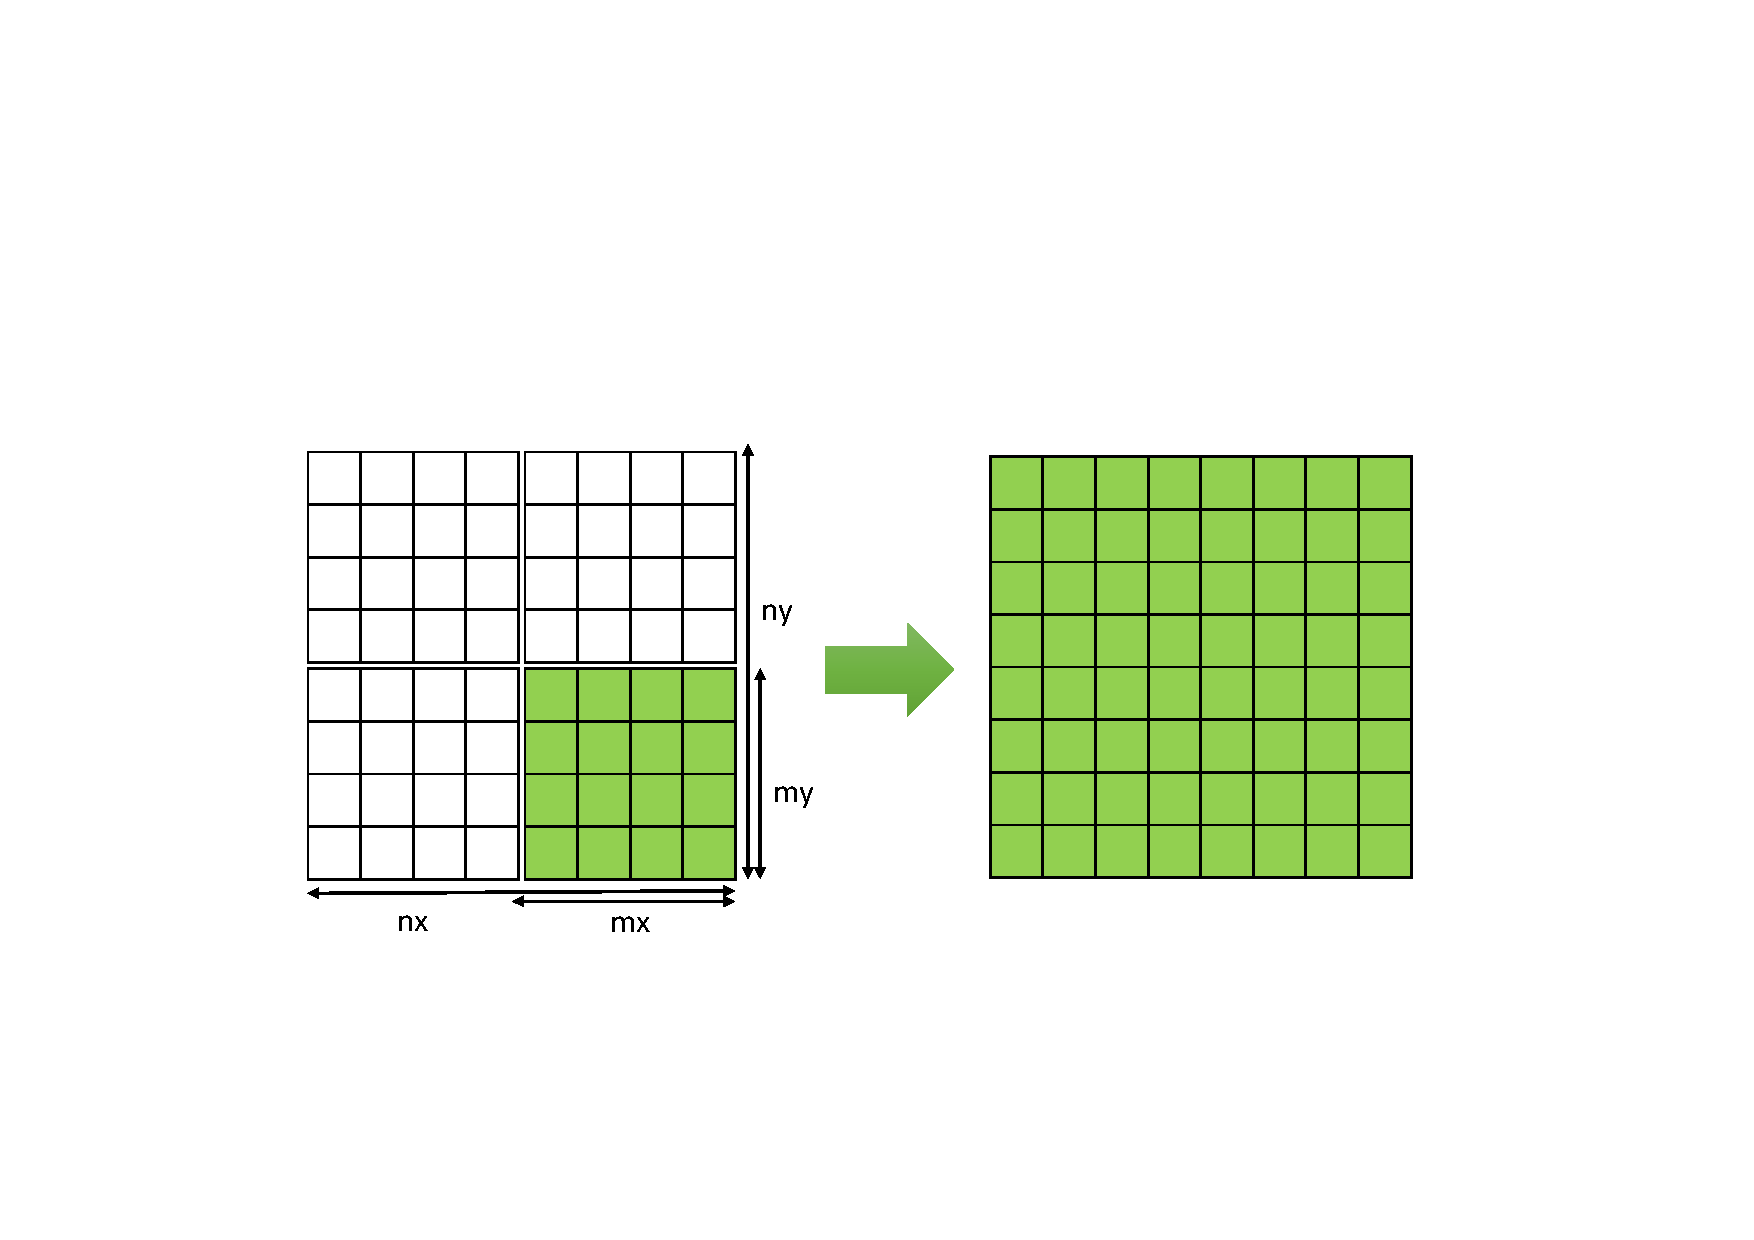
\includegraphics[width=0.9\textwidth]{Img/3PIC_combine.pdf}
    \caption{权重插值示意图}
    \label{fig:PIC_combine}
\end{figure}

上述为单GPU的权重差值方法,在使用多个GPU的时候,我们有两种方法:一种是使不同的GPU处理不同的空间域,在最后进行通讯,这种方法在CPU上的PIC程序中很常用,被称为“域分解”;另外一种是简单直接的使所有GPU做同样的工作,我们称这种模式为“复制模式”。
下面,我们使用一个例子对这两种方法进行比较,假设使用$64 \times 64 \times 64$个格点,区块大小为4*4*4,区块的数目为$16 \times 16 \times 16$,在TITAN上使用4个GPU运行。

\subsubsection{域分解模式}
在域分解模式中,每个GPU只需要处理相对应的域。假如区块数目为 $16 \times 16 \times 16$, 在4个GPU上运行的话,每个GPU需要处理的域的大小为$4 \times 16 \times 16$。但是,这种模式需要预先将粒子排序,使每个GPU只处理对应空间域内的粒子,因此需要额外的通讯和计算,具体步骤如下:
\begin{enumerate}
  \item GPU之间的粒子排序
  \begin{enumerate}
    \item 挑选粒子,每个线程处理一个区块,因此我们共有$4 \times 16 \times 16$=1024个线程。然而,在TITAN上每个GPU有2688个核,线程数小于核数,我们无法充分使用GPU。
    \item GPU之间信息交换
    \begin{enumerate}
      \item 从GPU内存拷贝到CPU内存,共需要拷贝$4 \times 16 \times 16$*(nGPU-1) * nPtcMax个粒子,其中nPtcMax个粒子为最大传输粒子数。
      \item CPU和CPU之间的信息交换,我们使用MPI\_send/receive,共需要交换$4 \times 16 \times 16$* (nGPU-1) *nPtcMax个粒子。
      \item 从CPU内存拷贝到GPU内存,共需要拷贝$4 \times 16 \times 16$*(nGPU-1) * nPtcMax个粒子。
    \end{enumerate}
  \end{enumerate}
  \item GPU内部的粒子排序,每个GPU的区块数目为$4 \times 16 \times 16$=1024,小于在每个 GPU 上的核数2688。
  \item GPU内部的权重差值,由于第一步进行了GPU之间的粒子排序,所以每个 GPU 上的粒子数目不同,格点数目为16*64*64。
  \item GPU之间的格点信息归约。
  \begin{enumerate}
    \item 从GPU内存拷贝到CPU内存,共需要拷贝16*64*64个格点。
    \item CPU和CPU之间的信息交换,我们使用MPI\_Allgether,共需要交换$64 \times 64 \times 64$个格点。
    \item 从CPU内存拷贝到GPU内存,共需要拷贝 $64 \times 64 \times 64$个格点。
  \end{enumerate}
\end{enumerate}

\subsubsection{复制模式}
在复制模式中,每个GPU进行同样的工作,同域分解模式相比,复制模式无法使用多GPU来节省计算时间,但是也无需在GPU之间进行粒子信息的交换。其流程如下所示,其中每一项和上面域分解模式相对。

\begin{enumerate}
  \item 无需GPU之间排序
  \item GPU内部的粒子排序,每个GPU的区块数目为$16 \times 16 \times 16$=4096,大于在每个 GPU上的核数2688。
  \item GPU内部的权重差值,每个GPU上的粒子数目相同。
  \item GPU之间的格点信息归约。
  \begin{enumerate}
    \item 从GPU内存拷贝到CPU内存,共需要拷贝$64 \times 64 \times 64$个格点。
    \item CPU和CPU之间的信息交换,我们使用MPI\_Allreduce,共需要交换 $64 \times 64 \times 64$个格点。
    \item 从CPU内存拷贝到GPU内存,共需要拷贝$64 \times 64 \times 64$个格点。
  \end{enumerate}
\end{enumerate}

可以看出,两个模式相比较的话,域分解模式在第一步中有了很多额外的通讯,在第二步与第三步中能够使用更少的格点数。然后,使用通讯时间来换取更少的计算量并不能带来效率的提升,而且,在域分解模式下,我们并不能充分利用GPU。因此,在我们的代码中以及接下来的性能测试中,我们均采用“复制模式”。

\subsection{泊松方程}
\label{section:PIC_GPU_Poisson}
在将粒子权重到网格上之后,下一步即解网格上的泊松方程。在单GPU上运行的版本我们在此不再赘述,而在多GPU上的并行版本和权重差值相似,也存在两种方法:一种是参考经典的CPU上的PIC程序,使用不同的GPU处理不同的空间域,即“域分解模式”;另外一种是简单直接的使所有GPU做同样的工作,即“复制模式”。由于解泊松方程的运算量较大,是PIC方法中很重要的一步,我们对两种模式都进行了实现并进行了比较。

\subsubsection{域分解模式与复制模式}
域分解的优点在于,通过使用不同的GPU处理不同的空间域,每个GPU可以降低计算量,从而提高程序运行速度;缺点也很明显,域分解模式需要不同GPU之间的信息交换,而在目前GPU与GPU之间,特别是在不同节点之间,并不能直接进行信息交换,而是必须通过CPU来进行,即信息交换需要三步:
\begin{enumerate}
  \item 从GPU内存拷贝到CPU内存。
  \item CPU和CPU之间的通过MPI进行信息交换。
  \item 从CPU内存拷贝到GPU内存。
\end{enumerate}

如小节\ref{section:PIC_FFT}所示,求解泊松方程中最主要的部分是使用傅里叶变换(FFT)。在GPU代码中,我们使用NVIDIA公司的CUDA快速傅里叶变换库(cuFFT)\cite{nvidia2010cufft}在进行变换。在求解多GPU上的3维傅里叶变换时,最好是在三个方向分别做1维的傅里叶变换,并在每次变换之间对数据进行转置。

假设在X,Y,Z三个方向上的格点数分别为$N_x$,$N_y$,$N_z$,那么当执行X方向的傅里叶变换的时候,变换的数组长度即为$N_x$,变换的次数为$N_y \times N_z$。 以使用四个GPU为例,那么1号GPU需要处理的数据为\verb'rho'[$N_x$][$0 \rightarrow \frac{N_y}{4}$][$N_z$],2号GPU需要处理的数据为\verb'rho'[$N_x$][$\frac{N_y}{4} \rightarrow 2\frac{N_y}{4}$][$N_z$],3号GPU需要处理的数据为\verb'rho'[$N_x$][$2\frac{N_y}{4}\rightarrow 3\frac{N_y}{4}$][$N_z$],4号GPU需要处理的数据为\verb'rho'[$N_x$][$3\frac{N_y}{4}\rightarrow N_y$][$N_z$]。每个GPU只需要进行$\frac{N_y}{4} \times N_z$ 次变换即可。理想情况下,和单GPU运行相比,使用4个GPU运行只需要花费1/4的时间。

在X方向的傅里叶变换结束后,我们需要其他的数据来进行Y方向的运算,目前每个GPU上的数据为\verb'rho'[$N_x$][$(n-1)\frac{N_y}{4}\rightarrow (n)\frac{N_y}{4}$][$N_z$],而进行Y方向的傅里叶变换需要的数据为\verb'rho'[$(n-1)\frac{N_x}{4}\rightarrow (n)\frac{N_x}{4}$][$N_y$][$N_z$]。我们必须对数据求转置并在GPU之间进行数据交换。而由于目前GPU与GPU之间并不能直接进行数据交换,我们不需将GPU中的数据拷贝回CPU内存中,并在CPU端进行通讯,这将需要额外的时间。所以域分解模式相比复制模式的效率高低将取决于额外的通信时间与降低的运算时间的比较。

以$64 \times 64 \times 64$个格点数,使用4个GPU为例,域分解模式求解泊松方程的具体步骤可以表示如下:
\begin{enumerate}
  \item X方向的FFT
  \begin{enumerate}
    \item 拷贝到GPU(64*16*64)
    \item FFT(64*16*64)
    \item 拷贝到CPU(64*16*64)
  \end{enumerate}
  \item 转置及CPU与CPU之间的信息通讯
  \item Y方向的FFT
  \begin{enumerate}
    \item 拷贝到GPU(64*16*64)
    \item FFT(64*16*64)
    \item 拷贝到CPU(64*16*64)
  \end{enumerate}
  \item 转置及CPU与CPU之间的信息通讯
  \item Z方向的FFT
  \begin{enumerate}
    \item 拷贝到GPU(64*16*64)
    \item FFT(64*16*64)
    \item 拷贝到CPU(64*16*64)
  \end{enumerate}
\end{enumerate}

相比较而言,复制模式的步骤为:
\begin{enumerate}
  \item X方向的FFT($64 \times 64 \times 64$)
  \item Y方向的FFT($64 \times 64 \times 64$)
  \item Z方向的FFT($64 \times 64 \times 64$)
\end{enumerate}
\subsubsection{单GPU测试}
我们在单GPU上对域分解模式进行了测试,并统计了每一部分所花费的时间。测试的格点数为$64 \times 64 \times 64$,每部分所花费的时间如表\ref{tab:1GPU_Poisson},表中的单位为秒,每部分占比如图\ref{fig:1GPU_Poisson}。

\begin{table}[!htbp]
    \centering
    \footnotesize% fontsize
    \setlength{\tabcolsep}{4pt}% column separation
    \renewcommand{\arraystretch}{1.2}%row space
    \begin{tabular}{lc}
        \hline\hline
        从CPU拷贝到GPU    & 1.306     \\
        \hline
        从GPU拷贝到CPU    & 2.979     \\
        \hline
        FFT计算           & 0.487     \\
        \hline
        转置和通讯        & 3.772     \\
        \hline
        总计              & 8.544    \\
        \hline\hline
    \end{tabular}
    \caption{单GPU域分解模式解泊松方程}
    \label{tab:1GPU_Poisson}
\end{table}

\begin{figure}[!htb]
    \centering
    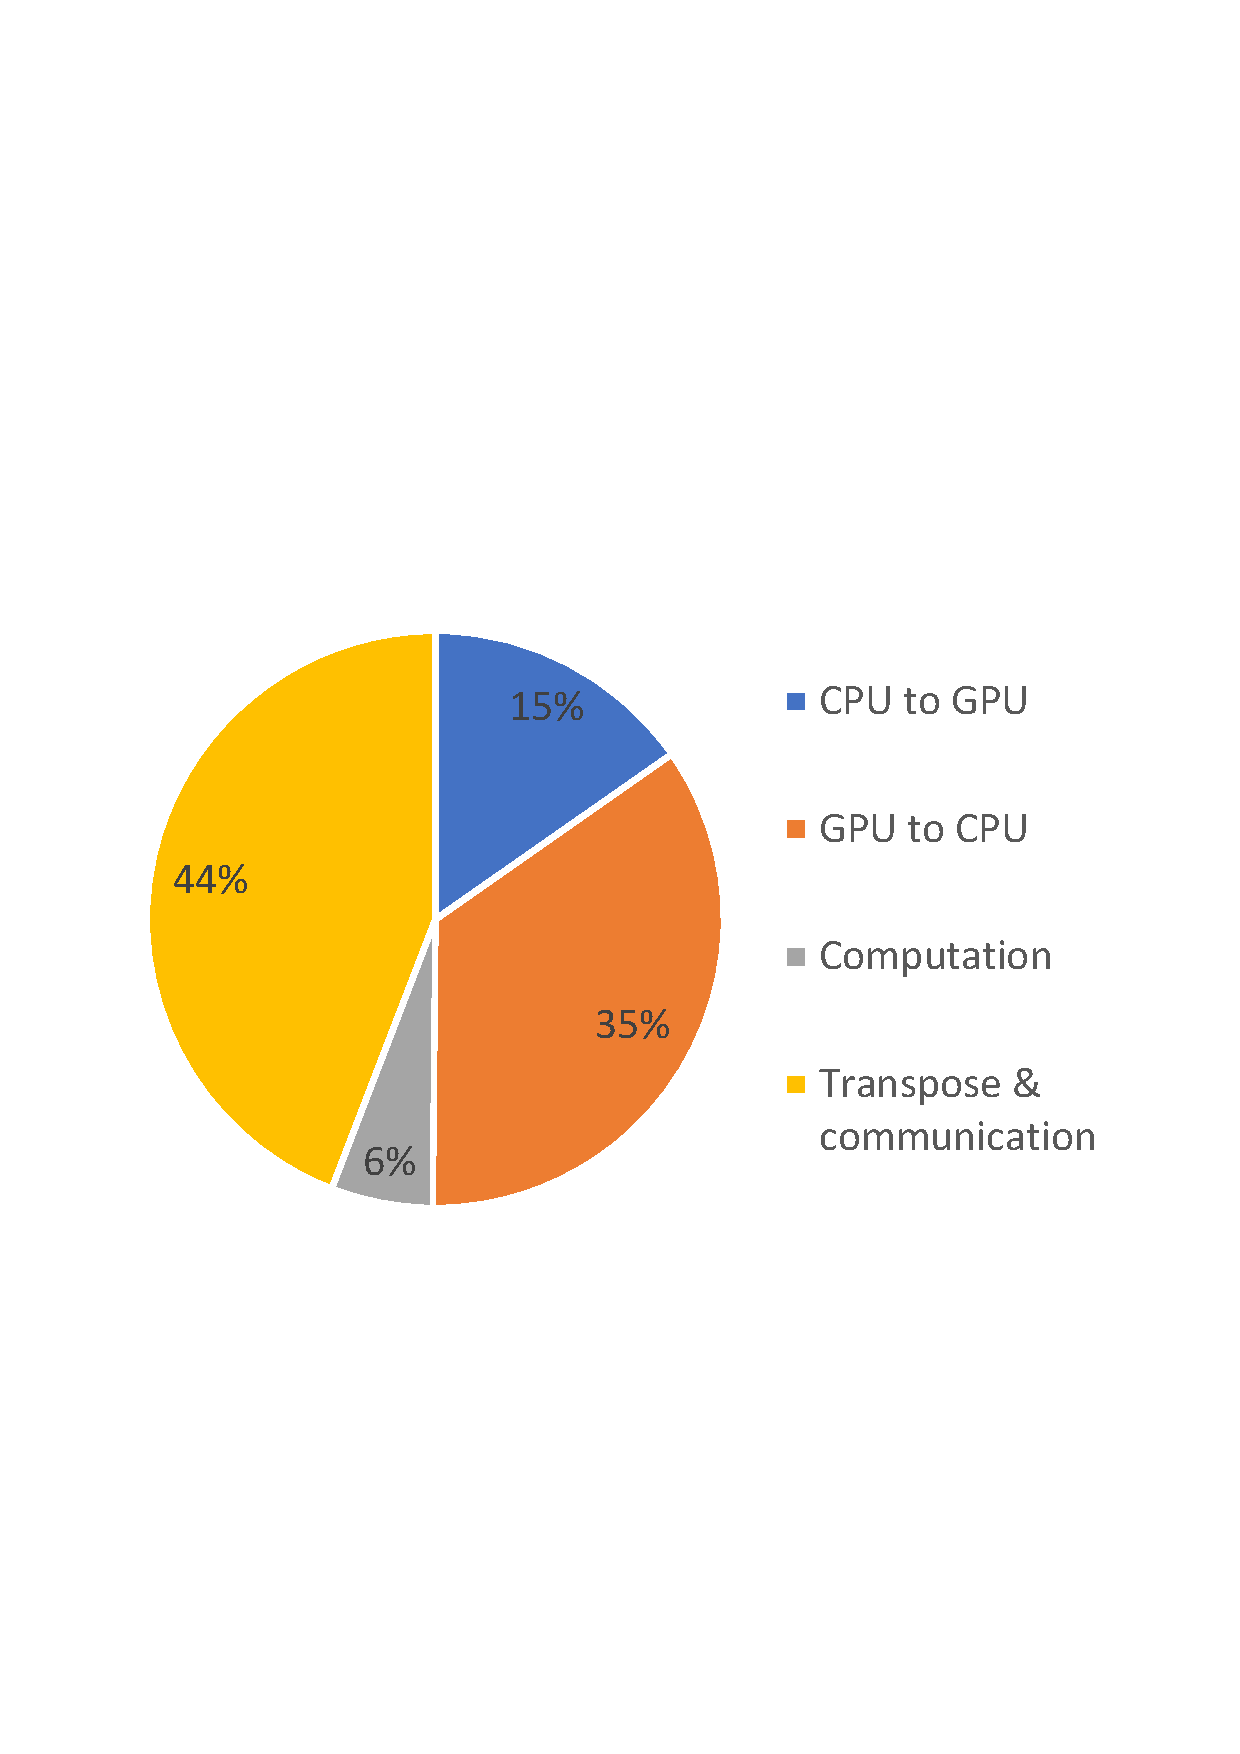
\includegraphics[width=0.7\textwidth]{Img/domain_decomposition_1GPU.pdf}
    \caption{单GPU域分解模式解泊松方程各部分时间占比}\label{fig:1GPU_Poisson}
\end{figure}

可以看出,FFT计算所花的时间为0.487秒,相比于额外增加的数据拷贝时间1.306 + 4.627 = 4.933秒,其占比非常小,仅仅占总时间的6\%。

多GPU的一种方式是使用同一节点内使用多个GPU,因为节点内的总线宽度限制,数据拷贝时间并不会随着使用GPU数目的增加而明显减少。而复制模式只需要花费FFT计算的时间,因为FFT计算花费的时间0.487秒远小于数据拷贝的时间4.933秒,所以即使在理想情况下使用N个GPU时FFT计算的时间减少到原来的1/N,域分解模式的总时间依然是比复制模式要大。

多GPU的另一种使用跨节点的多个GPU,即每个节点有1个GPU,通过使用多个节点来使用多个GPU,这也是目前超级计算机TITAN的运行模式。总线宽度会随着节点数增加而增加,所以数据拷贝时间会下降,假设其下降为现行的,即在N个节点上运行的话拷贝数据时间只有原来的1/N,则总时间将会是 $4.933/N+0.487/N$,如果我们想要取得优于复制模式的速度,即 $4.933/N+0.487/N<0.487$, GPU数目必须大于11。类似的,如果我们想要取得两倍的速度,GPU数目必须大于22。然而,这个计算忽略了CPU和CPU之间的通讯时间,一般来说,节点间的通讯时间随着节点数目增加而增加,因此我们很难取得理想情况的加速比。

下面,我们分别对节点内多GPU和跨节点GPU进行测试。

\subsubsection{单节点多GPU测试}
在同一节点中,我们进行了格点数为$64 \times 64 \times 64$的多GPU测试,表\ref{tab:2GPU_Poisson}是各个部分所花费的时间,以及和单GPU时的对比。可以看出,双GPU的总时间更大了,由8.544秒增加到了9.537秒。其中,FFT计算的时间有0.487秒减少到了0.249秒,几乎减少了一半,证明了多GPU对于减少纯FFT计算时间是确实有效的;对于数据拷贝时间,双GPU略有减少,大概减少了三分之一;总时间中增加的部分来源于转置和通讯的时间,几乎增加了一倍。
\begin{table}[!htbp]
    \centering
    \footnotesize% fontsize
    \setlength{\tabcolsep}{4pt}% column separation
    \renewcommand{\arraystretch}{1.2}%row space
    \begin{tabular}{lcc}
        \hline\hline
                          & 1GPU    & 2GPU   \\
        \hline\hline
        从CPU拷贝到GPU    & 1.306   & 0.817  \\
        \hline
        从GPU拷贝到CPU    & 2.979   & 1.991  \\
        \hline
        FFT计算           & 0.487   & 0.249  \\
        \hline
        转置和通讯        & 3.772   & 6.480  \\
        \hline
        总计              & 8.544   & 9.537  \\
        \hline\hline
    \end{tabular}
    \caption{单节点双GPU域分解模式解泊松方程}
    \label{tab:2GPU_Poisson}
\end{table}

\subsubsection{跨节点多GPU测试}
我们使用超级计算机泰坦(Titan)来进行域分解模式下的解泊松方程在跨节点多GPU上的效率。泰坦是一台由克雷公司承建的超级电脑,置放于美国能源部下属的橡树岭国家实验室中,使用由超微半导体提供的皓龙(Opteron)处理器链接英伟达提供的Tesla运算用GPU以进行协同运算。

首先,我们测试了常用的$64 \times 64 \times 64$个格点下,域分解模式下解泊松方程所花费的时间随GPU个数的变化,如图\ref{fig:TITAN_GPU_Poisson64}所示,图中蓝线为总时间,各个柱代表各个部分所花费的时间,在GPU数目很大时,图中不清楚部分可以参考表\ref{tab:TITAN_GPU_Poisson64}。

可以看出,花费的总时间随着GPU数目增加而逐渐减少,并在32个GPU的时候到达最小值,随后开始逐渐增加。其中,拷贝数据所花费的时间基本随着GPU的数目线性减少;而通讯所花费的时间先随着GPU数目增加而逐渐减少,到达极值后又开始逐渐增加,此时通讯时间占程序所花费的时间的绝大部分;FFT计算所花费的时间随着GPU数目的增加而逐渐减少,但是FFT计算占总时间的百分比很小。

\begin{figure}[!htb]
  \centering
  \begin{tabular}{|l|l|}
    \multicolumn{2}{c}{
    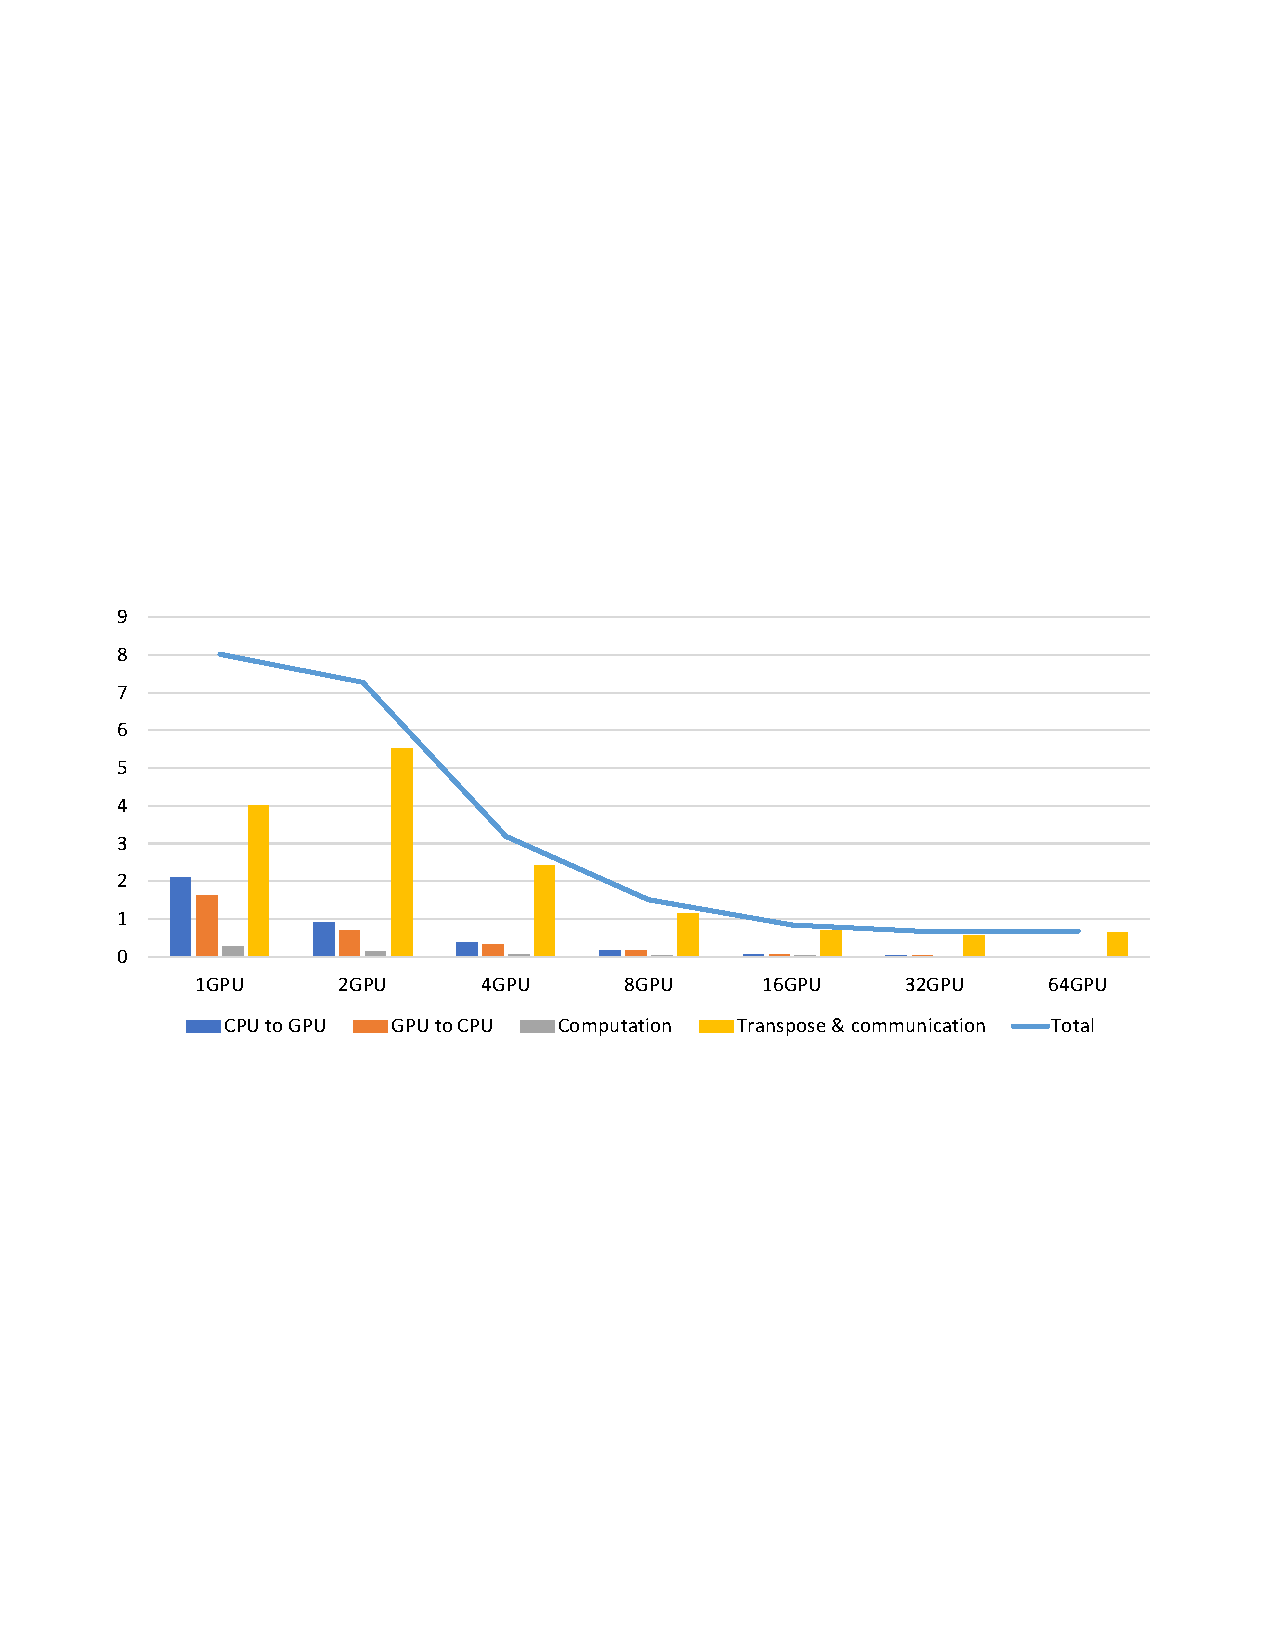
\includegraphics[width=0.9\textwidth]{Img/domain_decomposition_Titan64.pdf}} \\
  \end{tabular}
  \caption{$64 \times 64 \times 64$格点下,跨节点多~GPU~域分解模式解泊松方程时间随~GPU~个数的变化}
  \label{fig:TITAN_GPU_Poisson64}
\end{figure}

\begin{table}
  \centering
  \begin{tabular}{|l|c|c|c|c|c|c|c|}
    \hline
    GPU数目	    &1	    &2	    &4	    &8 	    &16	    &32  	&64   \\
    \hline
    CPU to GPU	&2.111	&0.922	&0.390	&0.158	&0.061	&0.031	&0.0155 \\
    GPU to CPU	&1.618	&0.694	&0.314	&0.167	&0.066	&0.033	&0.0158 \\
    FFT计算  	    &0.266	&0.136	&0.069	&0.039	&0.024	&0.017	&0.0150 \\
    转置和通讯	&4.02	&5.521	&2.415	&1.146	&0.691	&0.572	&0.6320 \\
    总计	        &8.015	&7.273	&3.188	&1.51	&0.842	&0.653	&0.6783 \\
    \hline
  \end{tabular}
  \caption{$64 \times 64 \times 64$格点下,跨节点多GPU 域分解模式解泊松方程各部分所用时间}
  \label{tab:TITAN_GPU_Poisson64}
\end{table}

我们也测试了更多格点数目时的情况,格点数目越多,所需要的计算量越大。当格点数为$128 \times 128 \times 128$时,程序在不同的GPU数目下消耗的时间如图\ref{fig:TITAN_GPU_Poisson128}和表\ref{tab:TITAN_GPU_Poisson128}所示,其整体的趋势和$64 \times 64 \times 64$时类似,因为更大的计算量,其总时间在使用128个GPU时到达最小值。

\begin{figure}[!htb]
  \centering
  \begin{tabular}{|l|l|}
    \multicolumn{2}{c}{
    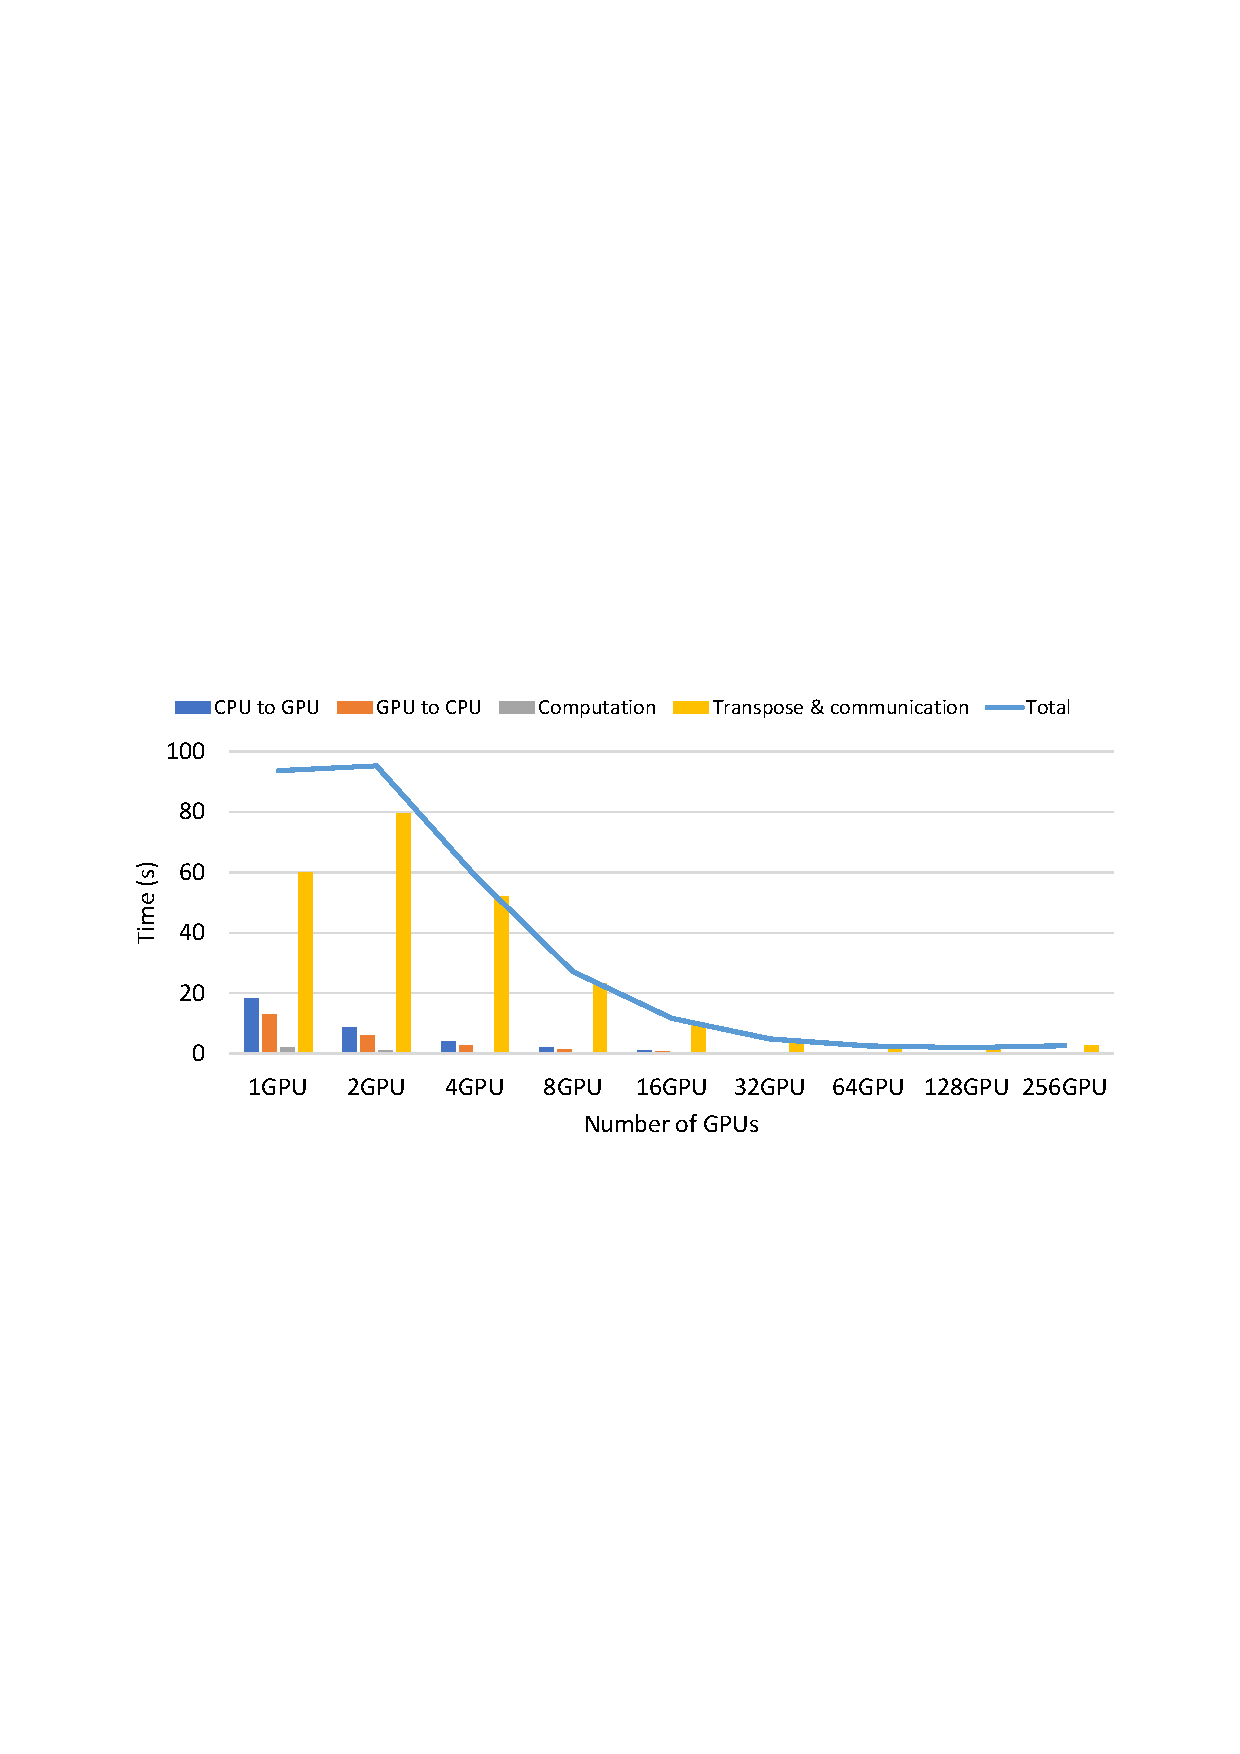
\includegraphics[width=0.9\textwidth]{Img/domain_decomposition_Titan128.pdf}} \\
  \end{tabular}
  \caption{$128 \times 128 \times 128$格点下,跨节点多~GPU~域分解模式解泊松方程时间随~GPU~个数的变化}
  \label{fig:TITAN_GPU_Poisson128}
\end{figure}

\begin{table}
  \centering
  \begin{tabular}{|>{\small}l|c|c|c|c|c|c|c|c|c|}
    \hline
    GPU数目	    &1	    &2	    &4	    &8 	    &16	    &32  	&64     &128	&256   \\
    \hline
    CPU to GPU	&18.29	&8.687	&3.946	&2.023	&0.953	&0.404	&0.148	&0.064	&0.033 \\
    GPU to CPU	&13.11	&6.15	&2.618	&1.463	&0.795	&0.368	&0.139	&0.07	&0.036 \\
    FFT计算  	&2.185	&1.034	&0.522	&0.266	&0.138	&0.071	&0.036	&0.021	&0.017 \\
    转置和通讯	&59.99	&79.34	&51.85	&23.30	&9.797	&4.041	&2.237	&1.859	&2.506 \\
    总计	    &93.58	&95.21	&58.94	&27.05	&11.68	&4.884	&2.56	&2.014	&2.592\\
    \hline
  \end{tabular}
  \caption{$128 \times 128 \times 128$格点下,跨节点多GPU域分解模式解泊松方程各部分所用时间}
  \label{tab:TITAN_GPU_Poisson128}
\end{table}

在$64 \times 64 \times 64$和$128 \times 128 \times 128$两种情况下,总时间开始都随着GPU数目增加而减小,然后到达最小值,随后由于通讯所需要的时间变大,总时间也随之变大。
\subsubsection{小结}
通过上面对于“域分解模式”的实现和测试,可以看出其主要受限于CPU和 GPU之间数据拷贝的速度与CPU和CPU之间的通讯速度。如果GPU带宽足够大,或者以后能够实现GPU与GPU之间的直接通讯的话,“域分解模式”可以作为一个可行的方案。但是在目前,与“复制模式”的比较,“域分解模式”由于其额外的数据拷贝和通讯开销,并不能通过减少运算量来达到提高速度的目的。所以我们在程序中依然使用“复制模式”,即使所有的GPU都同时运行同样的程序。

\subsection{粒子推动}
在小节\ref{section:PIC_GPU_depositor}粒子权重过程中,粒子是按照区块排列的。因此在推动粒子的时候,直接的方法是像权重过程中一样,由每个线程处理一个区块中的粒子。然而这种方法的缺陷是每个线程上的负载不均匀,可能出现某些区块中粒子数很多从而其线程运算量很大,然而另外某些区块中的粒子数较少,其线程运算量很小的情况。为了保证负载的均衡,我们采取另外一种方法,先把区块中的粒子信息重组,拷贝到一个典型的6*N的连续数组中,其中N是粒子数,6是维度;然后再并行推动。这种方法虽然需要额外的时间进行数据拷贝,但是相比第一种区块推动的负载更均匀,所以整体时间比区块推动更短,其流程如下所示:
\begin{enumerate}
  \item 将粒子从区块格式\verb"dev_ray_tile[lth*dim*npm*mth]" 重新排列,并拷贝到经典的6*N数组中\verb"dev_ray[N][6]"。
  \item 对\verb"dev_ray[N][6]"进行并行推动。
  \item 推动完成后,将粒子拷贝回原区块\verb"dev_ray_tile[lth*dim*npm*mth]" 中,以用来下一步的粒子排序和权重插值。
\end{enumerate}


\section{PIC算法在GPU上的正确性校验}
模拟程序最重要的确保模拟结果的正确性,我们通过将GPU程序的结果与成熟的CPU程序的结果进行比较来验证GPU程序的正确性。
图\ref{fig:PIC_GPU_benchmark}是CPU程序和~GPU~程序的发射度比较,从图中可以看出,两个程序得到的结果完全相同。通过输出数据得到,两者的区别在十的负十三次方量级,这可能是由于双精度浮点数的精度所限,双精度浮点数的精确度在十的负十四左右。而一般我们输出只取九位有效数字,所以可以认为两个程序的输出结果完全相同,GPU程序的正确性得到了验证。
\begin{figure}[!htb]
    \centering
    \begin{subfigure}[b]{0.9\textwidth}
        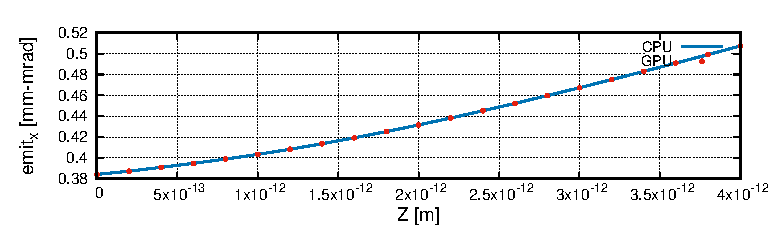
\includegraphics[width=\textwidth]{Img/PIC_GPU_benchmark_x.eps}
        %\caption{}
    \end{subfigure}
    \begin{subfigure}[b]{0.9\textwidth}
        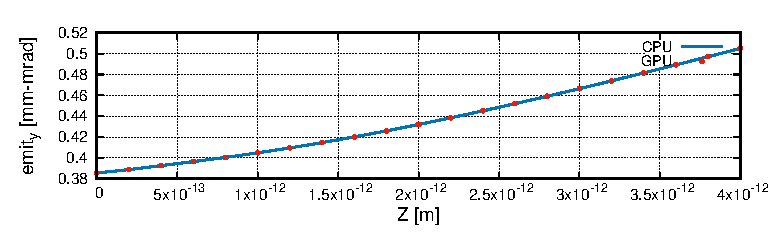
\includegraphics[width=\textwidth]{Img/PIC_GPU_benchmark_y.eps}
        %\caption{}
    \end{subfigure}
    \begin{subfigure}[b]{0.9\textwidth}
        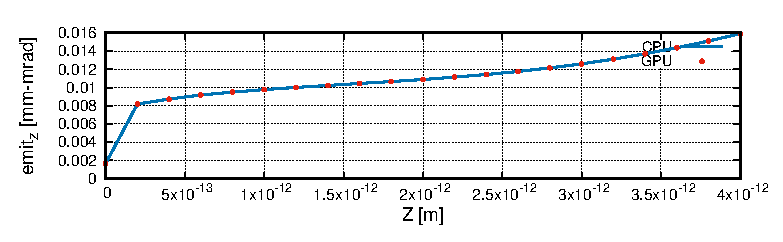
\includegraphics[width=\textwidth]{Img/PIC_GPU_benchmark_z.eps}
        %\caption{}
    \end{subfigure}
    \caption{PIC算法在GPU上的正确性校验}\label{fig:PIC_GPU_benchmark}
\end{figure}

\section{PIC算法在CPU集群上的实现}        \label{section:PIC_CPUcluster}
为了和GPU做比较,我们也在CPU集群上实现了PIC程序,其使用的计算机为Cori Knight Landing,使用的是Intel最新的众核处理器,每个处理器有68个核心。
我们的程序使用和MPI和OpenMP混合并行,以提高运行的效率。

首先,我们在一个节点上研究不同OpenMP线程数和MPI进程数下程序的效率和内存占用情况,并找到最优混合并行配置。之后,我们使用多个节点,研究程序在不同节点数下的效率变化。

\subsection{单节点}
首先,我们使用$64 \times 64 \times 64$个网格,在1.6m粒子数下测试不同的混合并行配置,如图\ref{fig:PIC_speedup_Cori_1node_1_6m}所示。其中横轴为不同的并行配置,MPI进程数由1指数增加到64,而~OpenMP~线程数有64指数得减小到1,线程数乘以进程数则保持不变。在每种并行配置下,总时间(浅蓝色实线),和权重差值,求解泊松方程,推动粒子,信息输出(各色柱行)所耗时间由左纵轴以秒为单位表示,而内存占用(绿色实线)由右纵轴以GB为单位表示。

\begin{figure}[!htb]
  \centering
  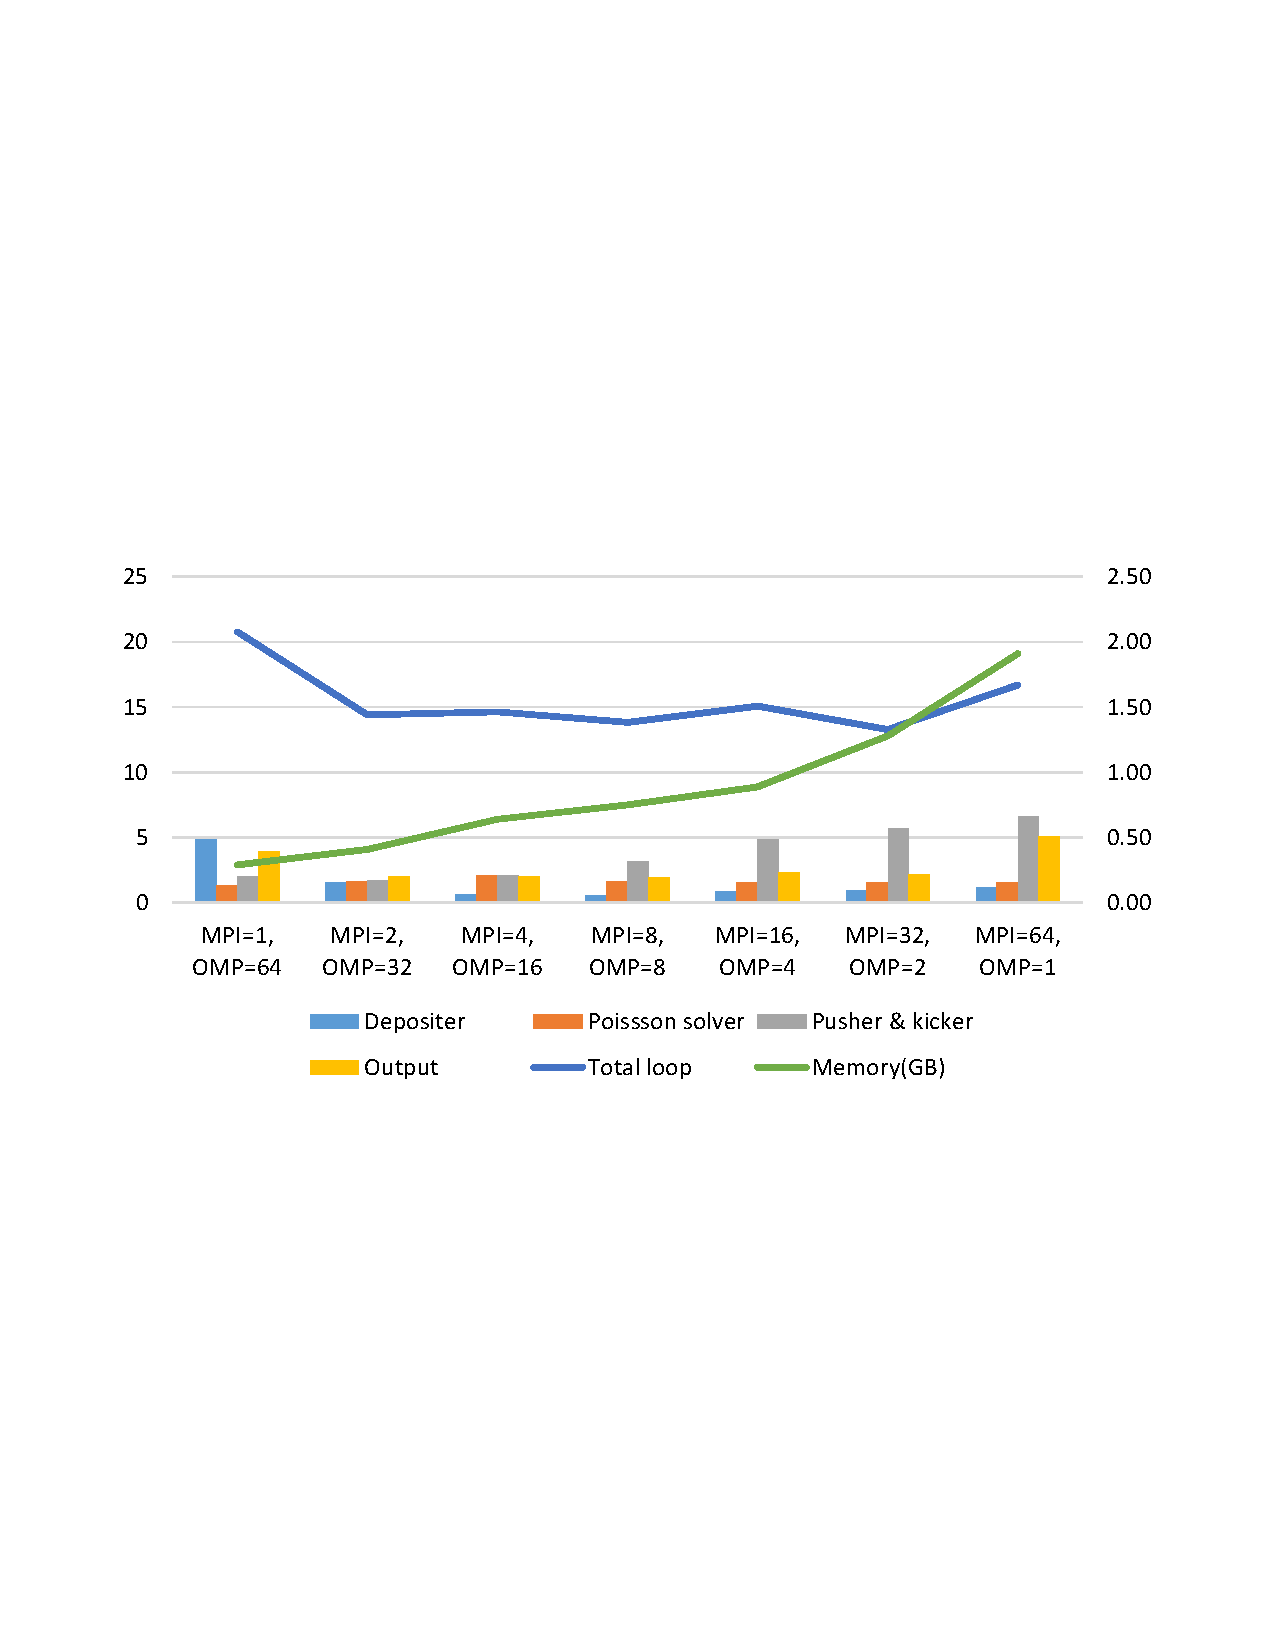
\includegraphics[width=0.9\textwidth]{Img/PIC_speedup_Cori_1node_1_6m.pdf}
  \caption{1.6m粒子数下,不同混合并行配置的耗时与内存占用}
  \label{fig:PIC_speedup_Cori_1node_1_6m}
\end{figure}

从图\ref{fig:PIC_speedup_Cori_1node_1_6m}可以看出,除了纯OpenMP并行(MPI=1,OMP=64)明显较慢外,其他各个并行配置下所消耗的总时间的差别并不大,
其中耗时最小的并行配置为使用32个MPI进程,每个进程使用2个OpenMP线程。一般而言,使用较大的MPI进程数是比较有效率的选择。
而内存占用基本随着MPI进程数目线性增加。



程序的不同部分对于并行配置的反应并不相同。随着MPI进程数的增加和每个进程所用线程数的减小,权重差值的耗时先减小后增加,一开始先从MPI=64,OMP=1时的1.14秒减少到了MPI = 8,OMP =8时的0.58秒,然后其开始剧烈增加,最终到达MPI = 1,OMP =64时的4.85秒。其原因是权重差值需要在不同的线程之间进行归约以避免线程冲突,而归约操作在线程数很大时有一个较大的启动时间。粒子推动耗时随着MPI数变大单调增加,这是因为OpenMP更适合Knight Landing众核架构,并能更有效的利用矢量处理器。

我们也测试了不同的粒子数下的并行配置,测试的粒子数为160k和16m,分别是之前粒子数的十分之一和十倍,其结果如图\ref{fig:PIC_speedup_Cori_1node_160k}和图\ref{fig:PIC_speedup_Cori_1node_16m}所示。
在160k个粒子的情况下,总时间随着MPI进程数的增加单调减少,这表明小粒子数情况更适合纯MPI并行。
而在1.6m个粒子的情况下,纯OpenMP并行由于无MPI进程间通讯,显示出一些优势,但是其总耗时依然大于MPI并行,其耗时最小的配置为MPI=64,OMP=1。

\begin{figure}[!htb]
  \centering
  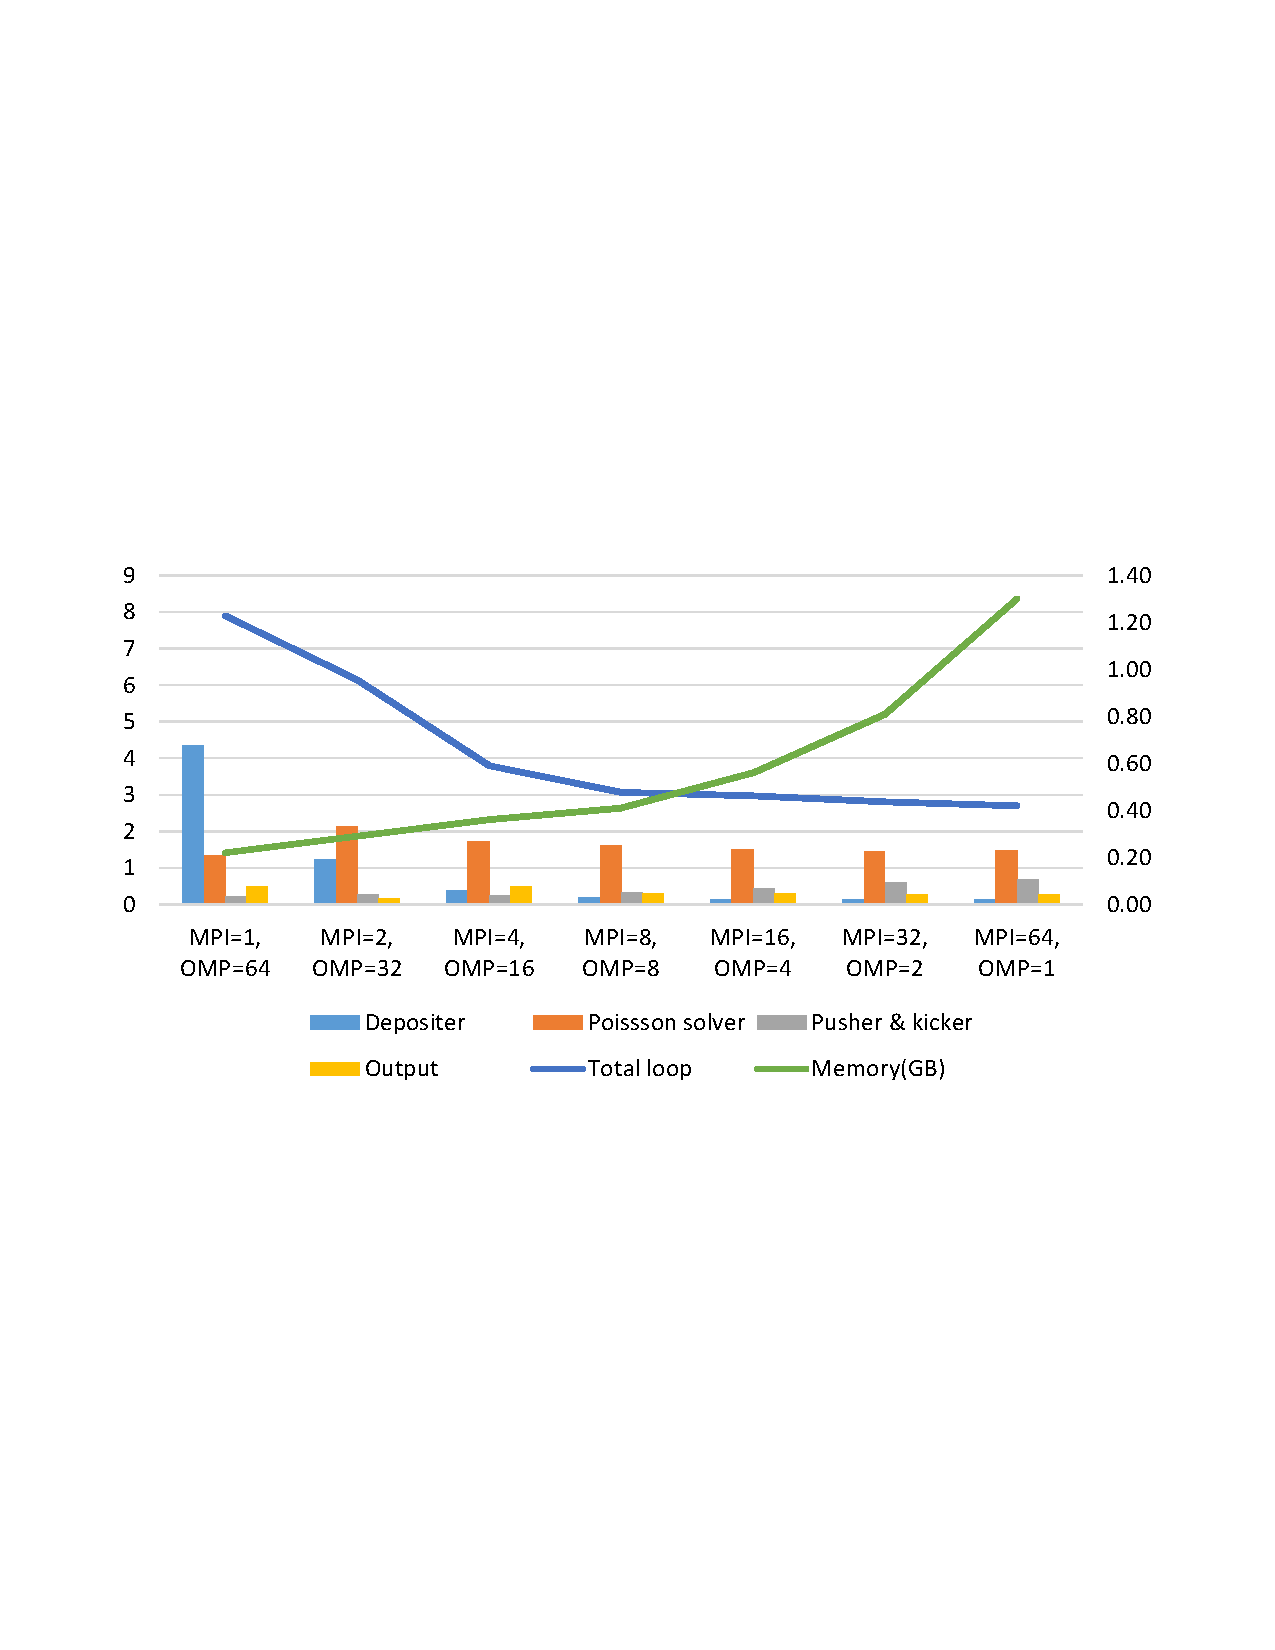
\includegraphics[width=0.9\textwidth]{Img/PIC_speedup_Cori_1node_160k.pdf}
  \caption{160k粒子数下,不同混合并行配置的耗时与内存占用}
  \label{fig:PIC_speedup_Cori_1node_160k}
\end{figure}

\begin{figure}[!htb]
  \centering
  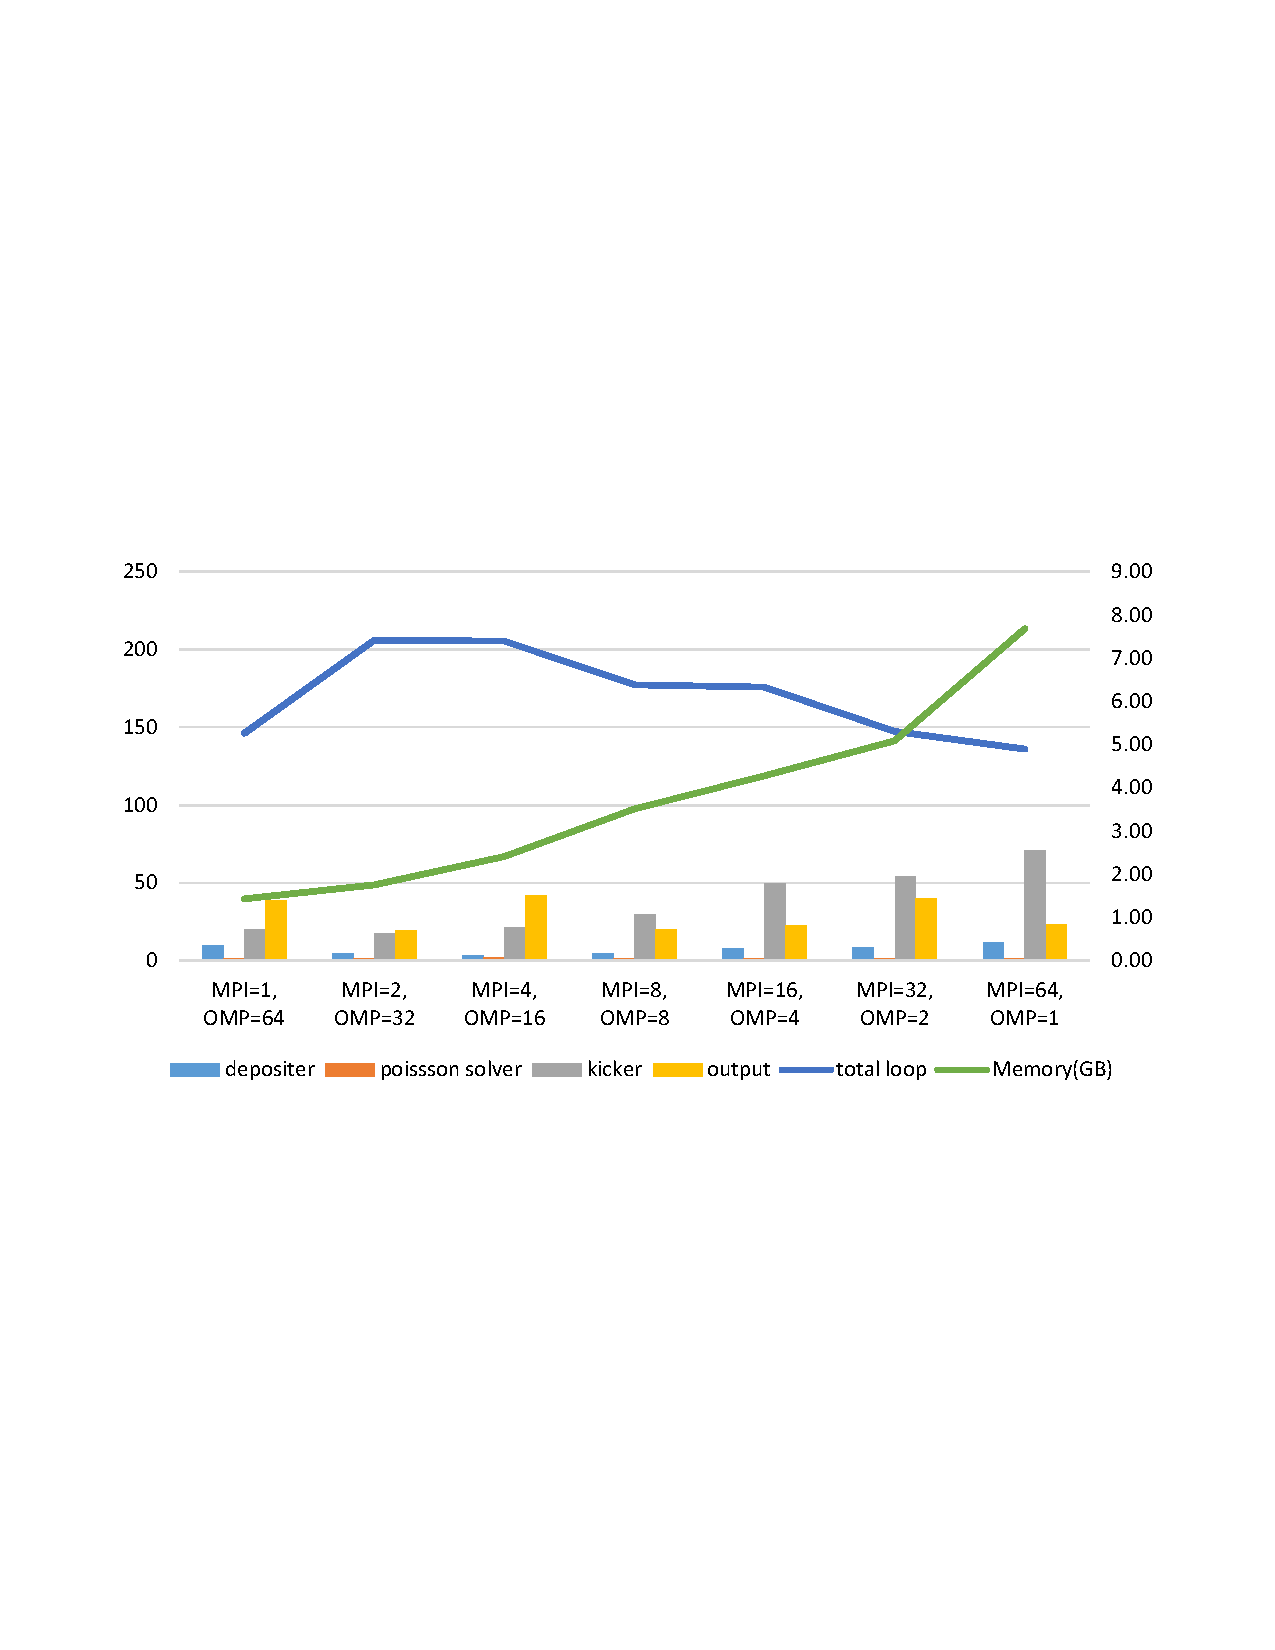
\includegraphics[width=0.9\textwidth]{Img/PIC_speedup_Cori_1node_16m.pdf}
  \caption{16m粒子数下,不同混合并行配置的耗时与内存占用}
  \label{fig:PIC_speedup_Cori_1node_16m}
\end{figure}

在各种情况下,无论粒子数多少,内存占用总是随着MPI进程数变大而单调增加。
\subsection{多节点}
从上面单节点的测试中可以得到,使用较大的MPI进程数和较小的OpenMP 线程数是更有效率的并行配置。
因此在多节点的测试中,我们首先选用纯MPI并行,测试在不同的节点数下程序总体以及各个部分的耗时情况。之后,我们也测试了OMP=2和OMP=4的情况,并与纯MPI程序进行了比较。

图\ref{fig:PIC_speedup_Cori_scalability}是纯MPI配置下PIC程序在CPU集群多节点下的耗时情况。每个节点我们使用64个核,图\ref{fig:PIC_speedup_Cori_scalability}的横轴为节点数目;左纵轴为时间,以秒为单位;右纵轴为内存使用,以GB为单位。随着使用更多的节点,程序总耗时先降低后增加,在32个节点处到达最小值。总耗时先减小是因为使用的节点数越多,每个节点上需要进行的运算越少;后增加是因为随着节点数上升,节点间的通讯时间也会随之增加。图\ref{fig:PIC_speedup_Cori_percetage_64nodes}为使用64个节点时程序各个部分消耗时间所占的百分比,可以看出此时通讯耗时已经占了总耗时的60\%。

\begin{figure}[!htb]
  \centering
  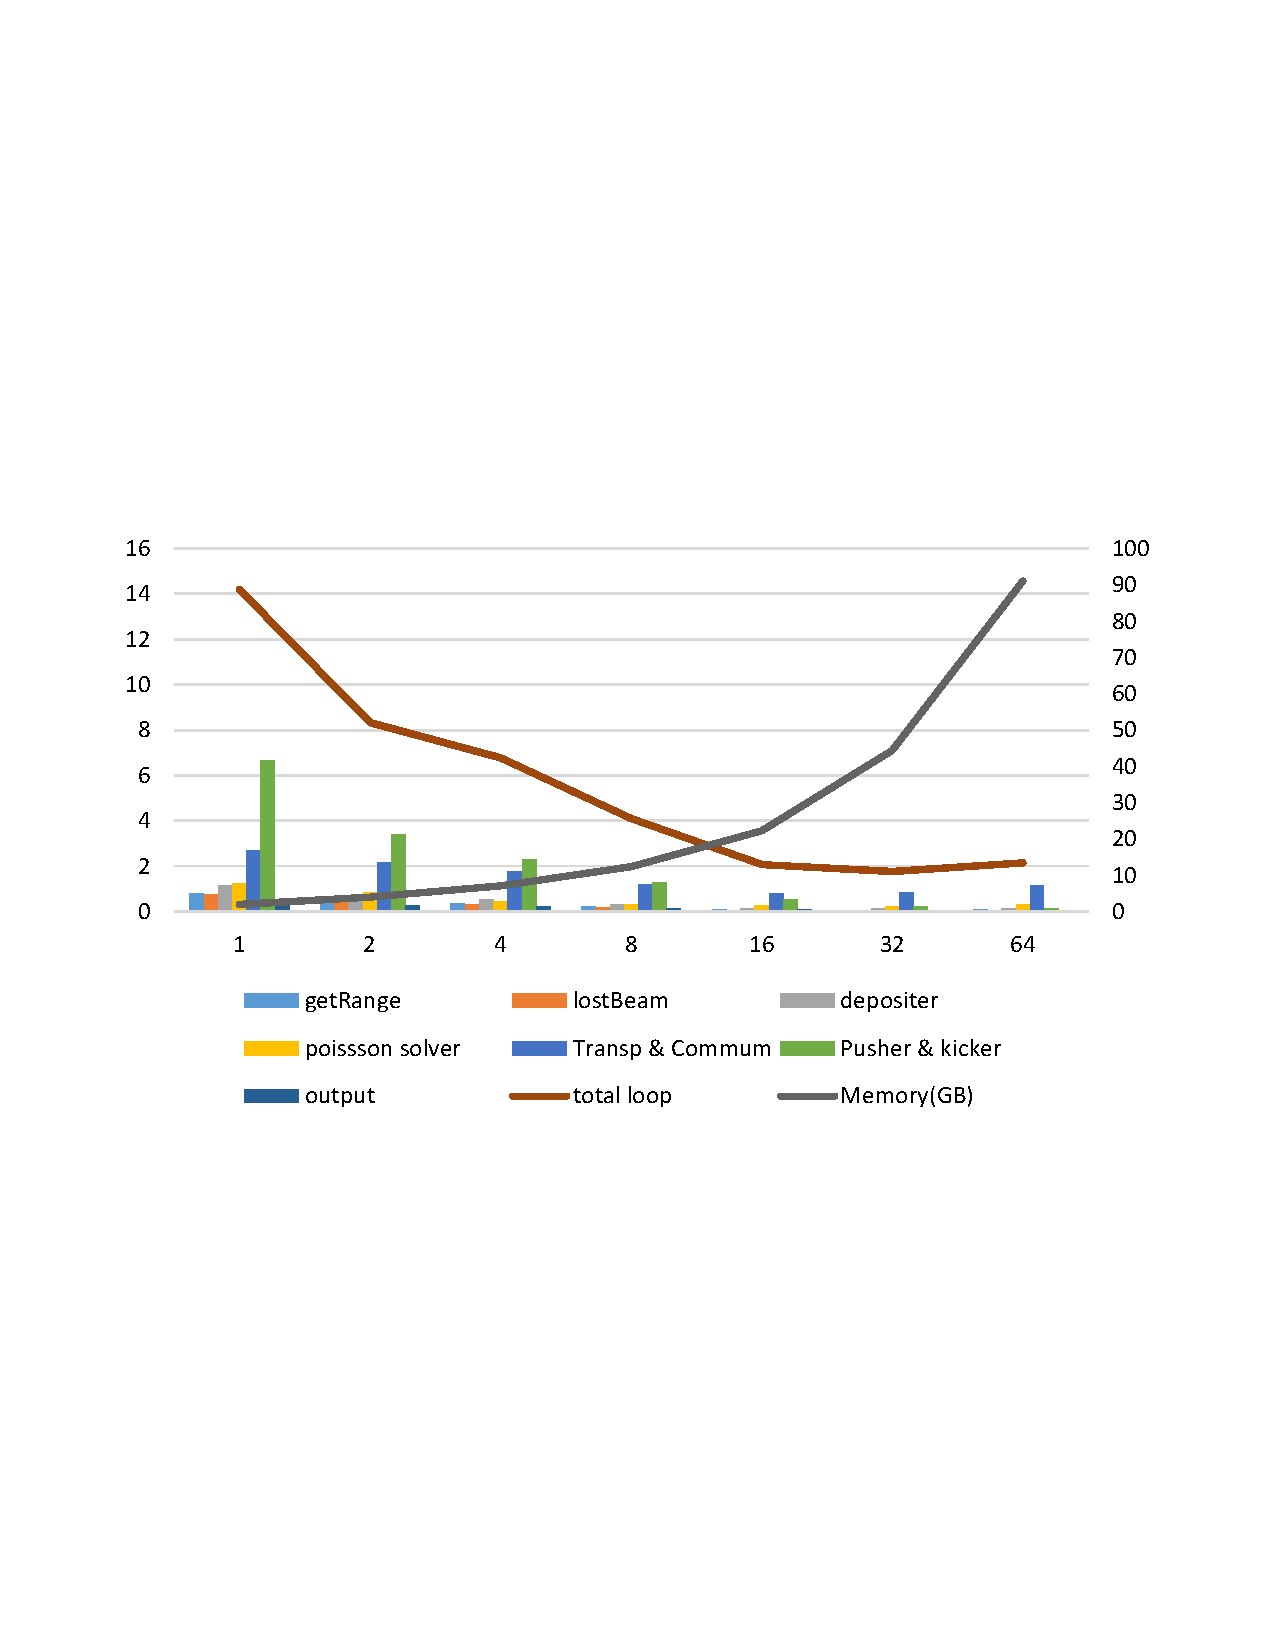
\includegraphics[width=0.9\textwidth]{Img/PIC_speedup_Cori_scalability.pdf}
  \caption{PIC程序使用多个CPU节点的耗时}
  \label{fig:PIC_speedup_Cori_scalability}
\end{figure}

\begin{figure}[!htb]
  \centering
  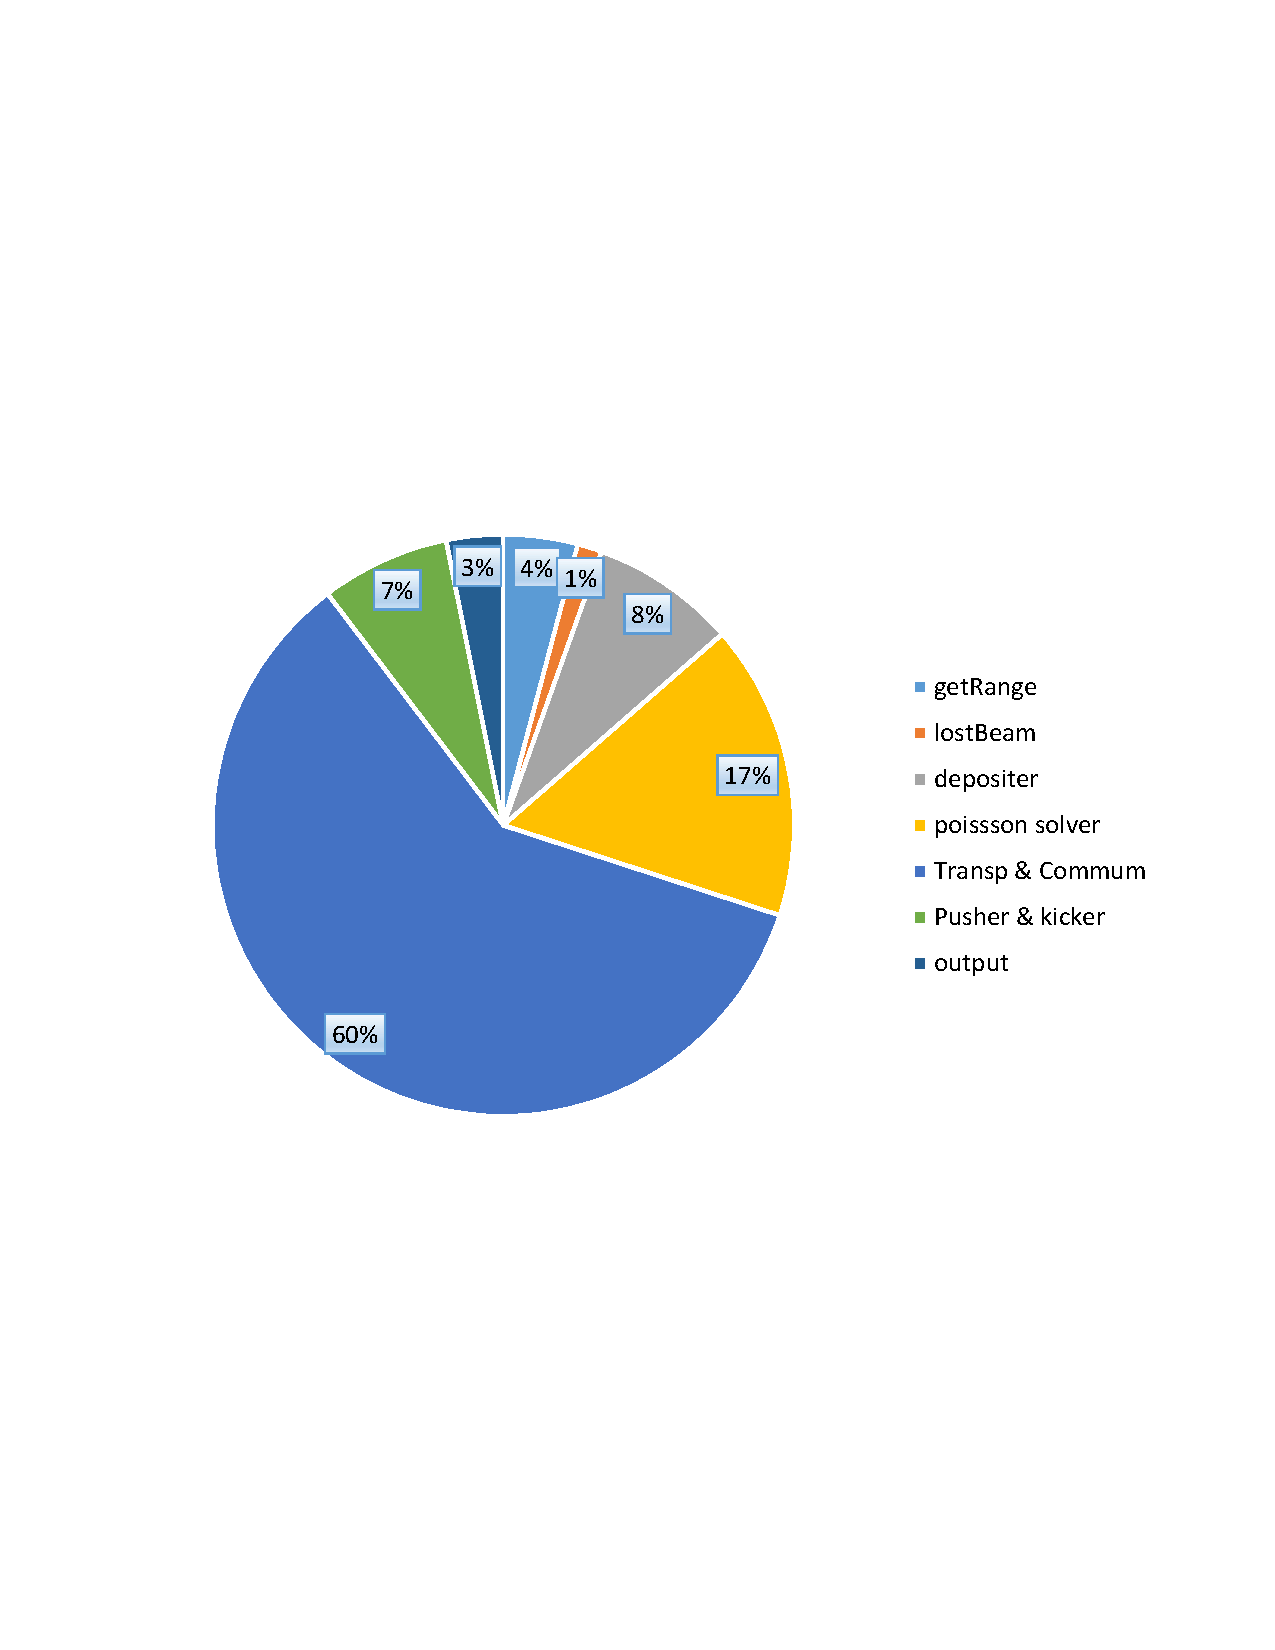
\includegraphics[width=0.5\textwidth]{Img/PIC_speedup_Cori_percetage_64nodes.pdf}
  \caption{使用64个节点时程序各个部分消耗时间所占的百分比}
  \label{fig:PIC_speedup_Cori_percetage_64nodes}
\end{figure}

接下来,我们对OMP=2和OMP=4的并行配置进行了测试,并与纯MPI程序(OMP=1)进行了比较,如图\ref{fig:PIC_speedup_Cori_multi_nodes_timeMemory}所示。
在大部分情况下,不同并行的耗时差别很小;但是在某些情况下差别很大,比如节点数为16时,纯MPI的速度是OMP=4的 1.8倍。
对于内存使用情况, 使用更多的OpenMP线程和更少的MPI进程总是占优势。
综合考虑,在内存足够大的情况下,在Knight Landing上运行的PIC程序使用纯MPI并行配置依然是一个很好的选择。

\begin{figure}[!htb]
    \centering
    \begin{subfigure}[b]{0.48\textwidth}
        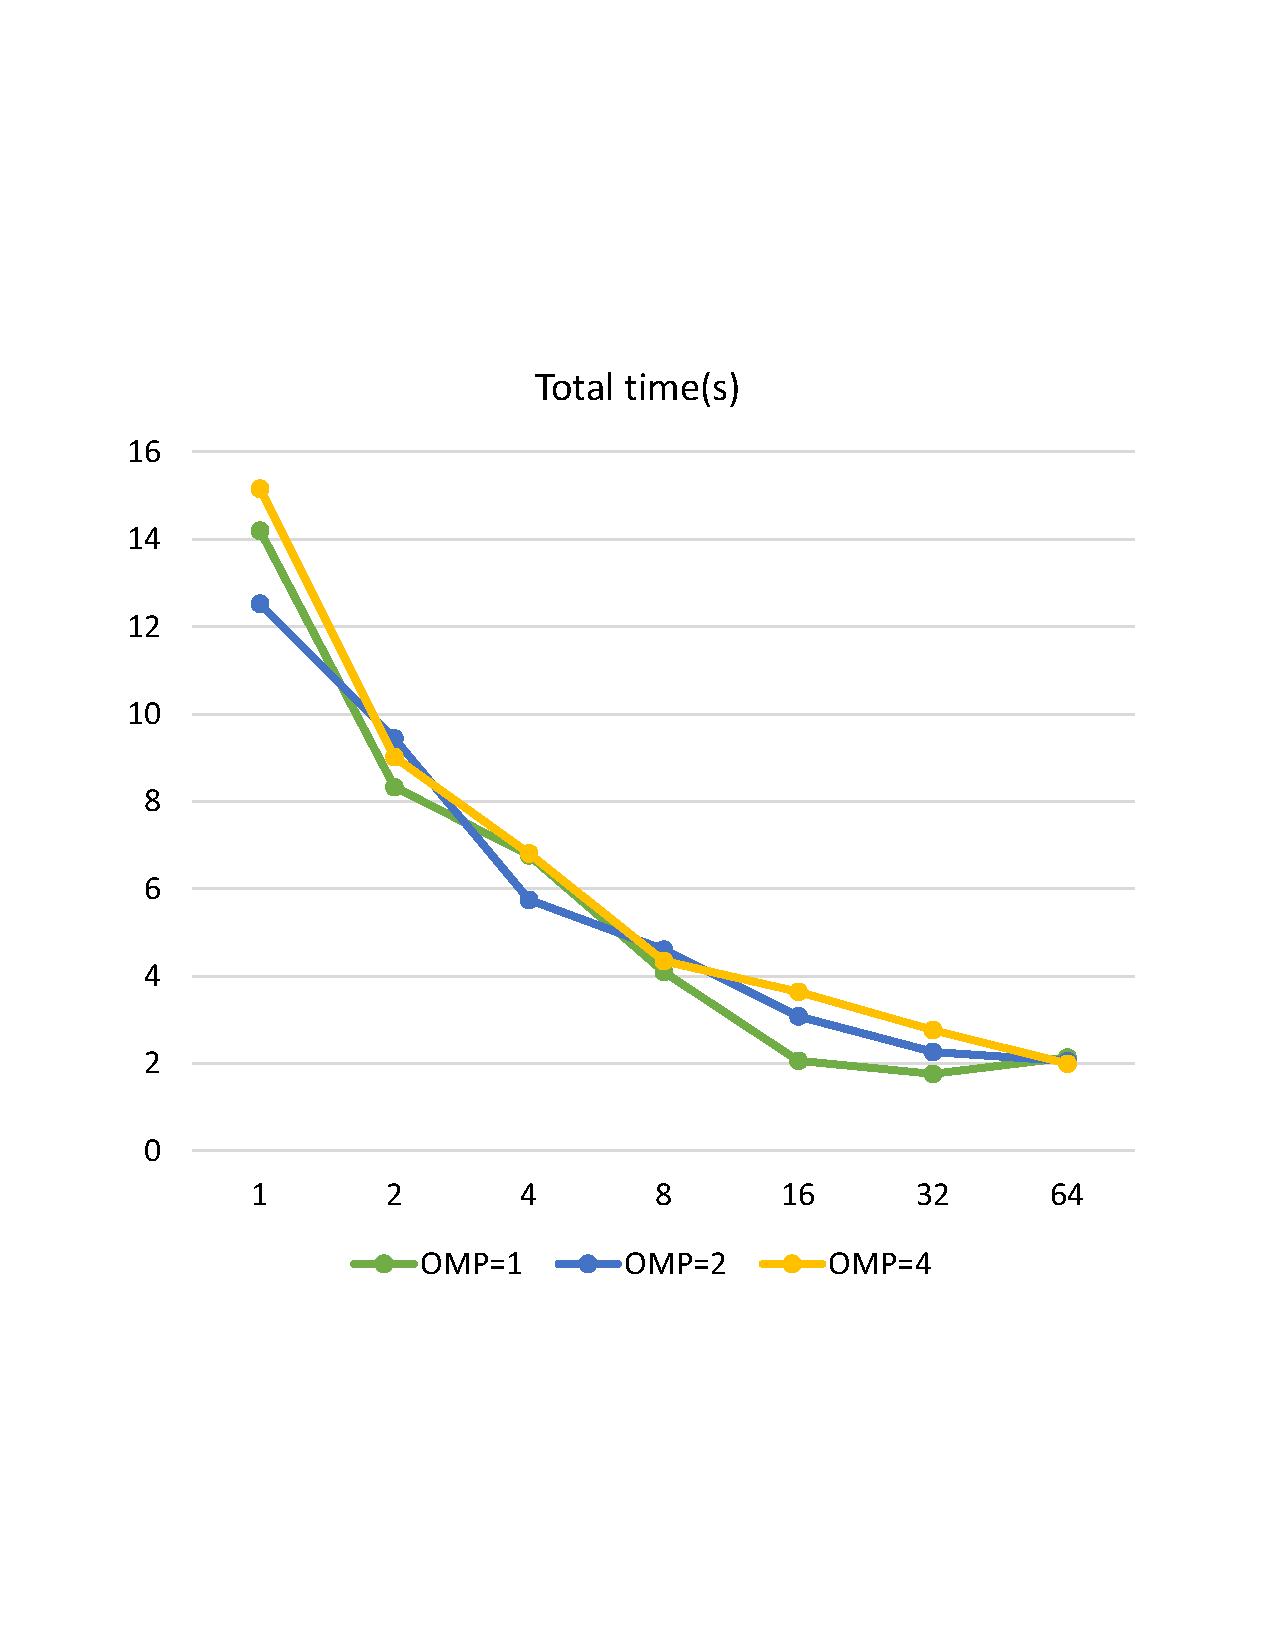
\includegraphics[width=\textwidth]{Img/PIC_speedup_Cori_multi_nodes_time.pdf}
        \caption{耗时}
    \end{subfigure}
    \begin{subfigure}[b]{0.48\textwidth}
        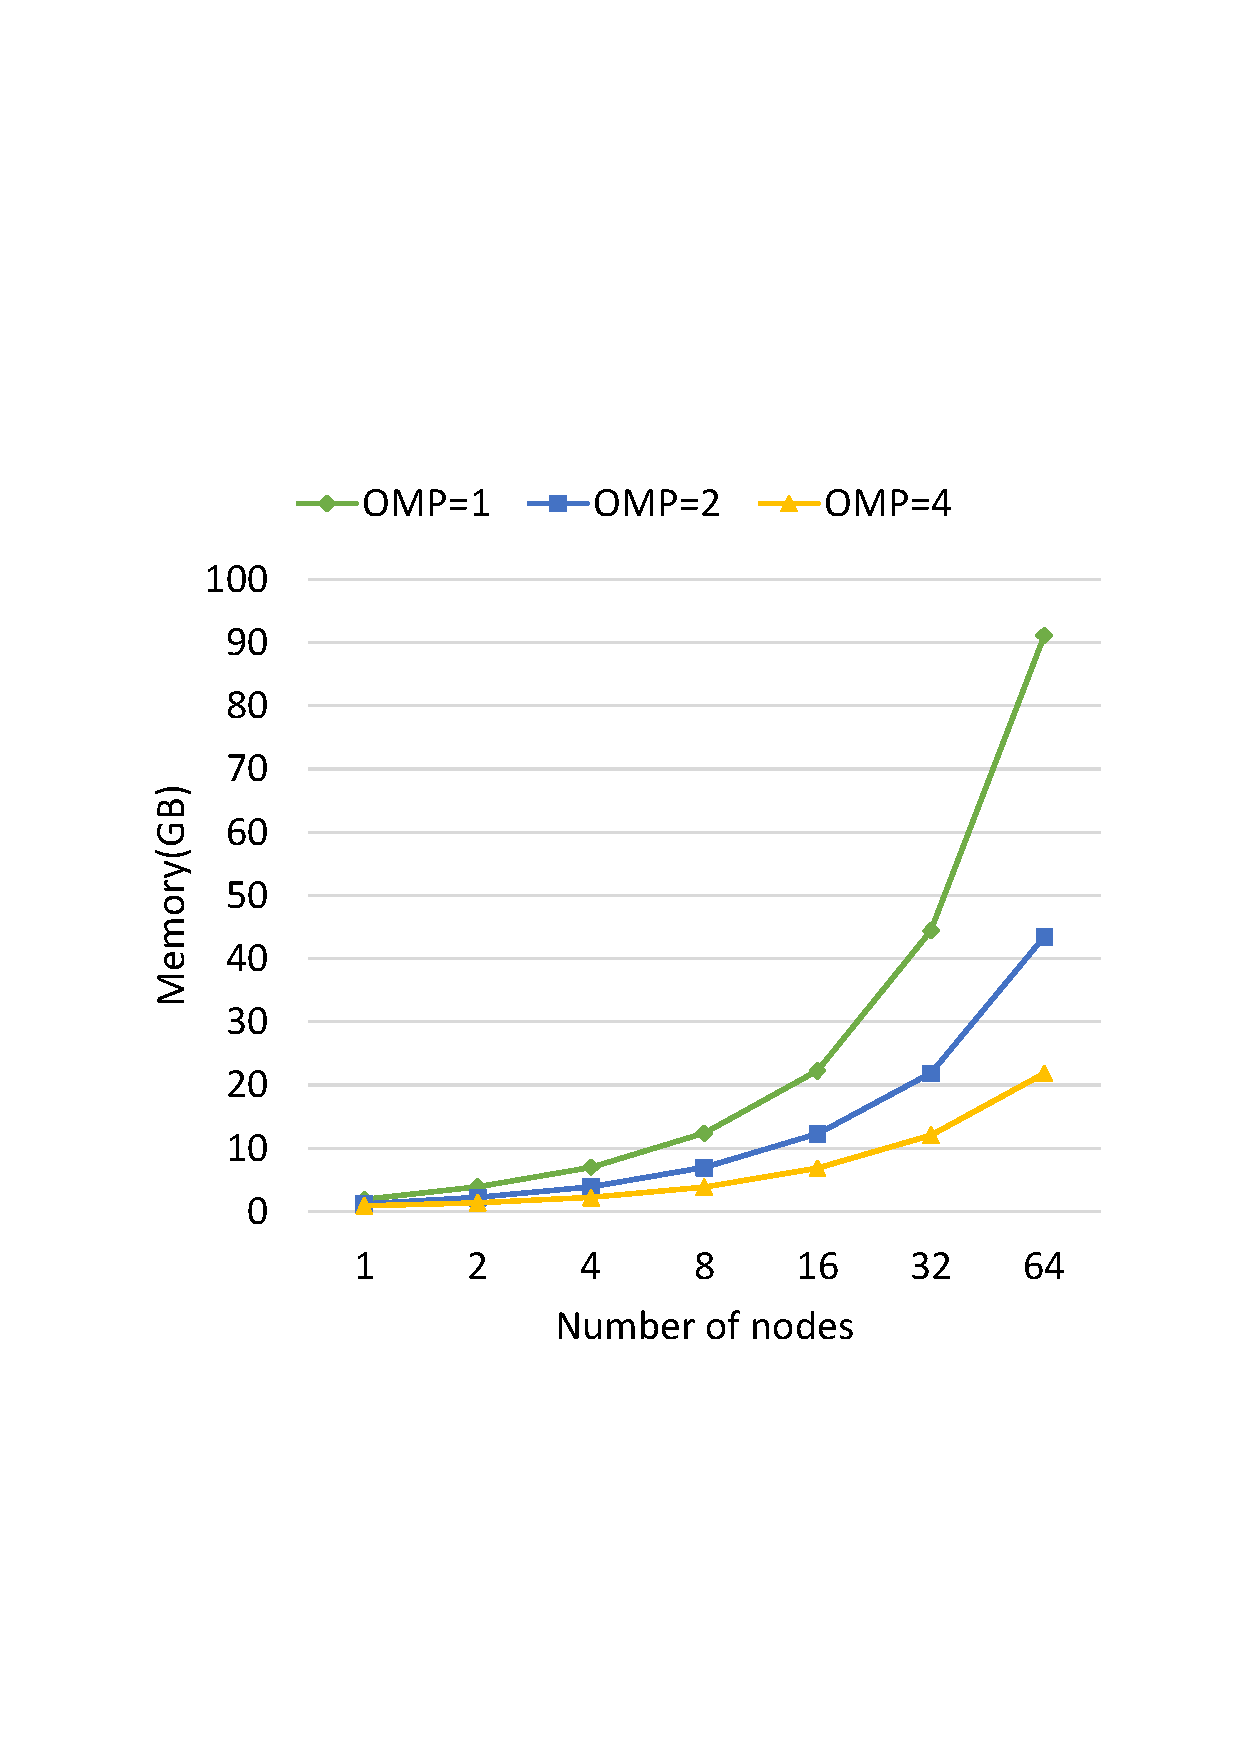
\includegraphics[width=\textwidth]{Img/PIC_speedup_Cori_multi_nodes_memory.pdf}
        \caption{内存占用}
    \end{subfigure}
    \caption{不同并行配置下的多节点运行情况比较}
    \label{fig:PIC_speedup_Cori_multi_nodes_timeMemory}
\end{figure}

\subsection{与GPU对比}

在本章之前的测试中,我们使用的GPU型号为Nvidia GeForce GTX 1060,其包含1280颗核心,时钟频率为1.71GHz。而我们使用的CPU型号为Intel® Xeon Phi™ Processor 7250 ("Knights Landing"),共包含68颗核心,时钟频率为1.40GHz,但是实际上,我们只是使用了64颗核心。

而由于GPU程序做了一些简化,缺少一部分步骤,例如粒子丢失判据等,我们在进行比较的时候也在CPU程序的耗时中减去了相应部分。
在$64 \times 64 \times 64$个格点数,1.6m个粒子的情况下,对于同样长度的加速器,使用一个GPU代码的总耗时为3.56秒,这类似于CPU程序在300个核心上的运行时间。换而言之,对于我们的PIC程序,一个GPU卡的运算效率与4到8个CPU节点的运行效率相当。


\section{Symplectic算法在GPU上的实现}     \label{section:symplectic_GPU}
Symplectic算法非常适合使用GPU进行加速计算。通过使用CUDA和GPU,可以显著加快无网格粒子跟踪代码的运行速度。当运行在单个GTX 1060时,与CPU串行相比,GPU代码实现了超过400倍的加速。此外,加速比会随着GPU的数目线性增长。
在大多数加速元件中,粒子会被推动若干步。在每一步中,粒子将首先被外场传输矩阵传输推动半个时间步长,然后由空间电荷推动一个时间步长,并再次被外场传输矩阵传输推动半个时间步长。
其中,求解空间电荷将消耗整个计算时间的90%以上。 计算空间电荷效应的程序由下面的三个子程序组成,而每个子程序由一个或两个内核组成。
\begin{enumerate}
  \item 遍历三角函数
  \item 计算$\Phi^{lmn}$
  \item 计算$ep_i$并推动粒子
\end{enumerate}

我们对程序进行了许多优化,使其更适合GPU架构,程序的性能得到显着改善。 每个子程序的优化策略各不相同,下面介绍各个内核的详细优化策略。
\subsection{遍历三角函数}
根据粒子的位置,我们首先计算每个粒子的三角函数临时变量。设:
\begin{equation}
\begin{array}{cc}
    S^{l}_j =sin(\alpha_l x_j), & C^{l}_j =cos(\alpha_l x_j)  \\
    S^{m}_j =sin(\alpha_m x_j), & C^{m}_j =cos(\alpha_m x_j)  \\
    S^{n}_j =sin(\alpha_n x_j), & C^{n}_j =cos(\alpha_n x_j)  \\
\end{array}
\end{equation}
其中下标$j$是指不同的粒子,下标$l$,$m$和$n$是指三个方向的频谱模式。

然后,X方向上的传输矩阵$ m_2 $(等式\ ref {eq:map1})可以表示为:
\begin{equation}\label{eq:map2}
{{p}_{xi}}(\tau )={{p}_{xi}}(0)-\tau \frac{1}{{{\varepsilon }_{0}}}\frac{8}{abc}\omega \kappa {{\gamma }_{0}}\sum\limits_{j=1}^{{{N}_{j}}}{\sum\limits_{l=1}^{{{N}_{l}}}{\sum\limits_{m=1}^{{{N}_{m}}}{\sum\limits_{n=1}^{{{N}_{n}}}{\frac{{{\alpha }_{l}}S_{j}^{l}S_{j}^{m}S_{j}^{n}C_{i}^{l}S_{i}^{m}S_{i}^{n}}{(\alpha _{l}^{2}+\beta _{m}^{2}+\gamma _{n}^{2})}}}}}
\end{equation}

与等式\ref{eq:map1}相比,新的传输矩阵节省了很大的计算量。
计算$ S_ {j} $和$ C_ {j}$是非常有必要的,这样可以避免后期处理的重复计算。在这个子程序中,我们采用按照粒子分配线程的策略,即每个线程处理一个粒子,这段程序结构相对简单,只占整个空间电荷效应求解所需时间的2%左右。 然而,它生成了$ 2 \times({{N}_{l}} + {{N}_{m}} + {{N}_{n}})\times {{N} _ {j}} $ 的数据,占了大部分的内存空间,而GPU的内存大小在给定型号的情况下是一个固定值,并不能通过添加内存条来增加,在这个意义上,这段程序决定了模拟中粒子数目的最大值,是花费存储空间以节省计算量而的典型示例。根据我们的测试,考虑到不可避免的内存碎片,假设展开阶数为$64\times64\times64$,程序可以在GeForce GTX 1060 6GB上处理大约100万个粒子。

由于需要遍历内存,该子程序的速度受到全局内存带宽的限制。为了改进内存读写,粒子数据是以阵列结构(SoA)排列的形式而不是结构数组(AoS),以达到对齐读取(coalesced memory read)。并且,在CPU侧分配页锁存存储器,以实现 CPU与GPU之间的数据复制速度更快。

\subsection{计算$\Phi^{lmn}$}\label{section:phi}
我们注意到在传输矩阵\ref{eq:map2}中,对下标$j$的求和是对每个粒子的求和,我们可以改变求和的顺序以节省计算量。如果我们定义:
\begin{equation}
\Phi^{lmn}\equiv \sum\limits_{j=1}^{{{N}_{j}}}{S_{j}^{l}S_{j}^{m}S_{j}^{n}}
\end{equation}

如果首先完成${{N}_{l}}\times{{N}_{m}}\times{{N}_{n}}$个$\Phi^{lmn}$的计算。传输矩阵\ref{eq:map2}可以重写为:

\begin{equation}\label{eq:map3}
{{p}_{xi}}(\tau )={{p}_{xi}}(0)-\tau \frac{1}{{{\varepsilon }_{0}}}\frac{8}{abc}\omega \kappa {{\gamma }_{0}}\sum\limits_{l=1}^{{{N}_{l}}}{\sum\limits_{m=1}^{{{N}_{m}}}{\sum\limits_{n=1}^{{{N}_{n}}}{\frac{\Phi^{lmn}{{\alpha }_{l}}C_{i}^{l}S_{i}^{m}S_{i}^{n}}{(\alpha _{l}^{2}+\beta _{m}^{2}+\gamma _{n}^{2})}}}}
\end{equation}

以这种方式,计算复杂度从$\alpha N_p^2*N_{modes}$减少到了$\alpha  N_p*N_{modes}$,这使这个保辛粒子跟踪算法的计算量大大降低。

该子程序的目的是为每个展开模计算$\Phi^{lmn}$,自然地我们使用每个线程处理一个模的方式。
然而,在通常情况下,我们使用$16\times 16\times 16$模式就可以得到收敛的结果,也就是说会有$16\times 16\times 16 = 4096$个线程,而GPU通常具有几百甚至几千个核心,这个线程数量相对于的GPU的核心数目来说较少。
为了实现负载平衡,我们将粒子分为几个部分,并采用CUDA流技术来获得高并发性。我们定义临时变量$\Phi^{lmn}_{temp,i}$:
\begin{equation}
\Phi^{lmn}_{temp,i}\equiv \sum\limits_{j=Nstar{{t}_{i}}}^{Nen{{d}_{i}}}{S_{j}^{l}S_{j}^{m}S_{j}^{n}}
\end{equation}
那么,$\Phi^{lmn}$由以下求和得到:
\begin{equation}
\Phi^{lmn}=\sum\limits_{i}{\Phi^{lmn}_{temp,i}}
\end{equation}

这个子程序的速度也是受到内存带宽的限制。我们在计算$Phi^{lmn}$之前,会首先对$S_{j}$进行转置以达到对齐读取。

\subsection{计算$ep_i$并推动粒子}
以x方向为例,我们定义:
\begin{equation}
ep{_{xi}}\equiv \tau \frac{1}{{{\varepsilon }_{0}}}\frac{8}{abc}\omega \kappa {{\gamma }_{0}}\sum\limits_{l=1}^{{{N}_{l}}}{\sum\limits_{m=1}^{{{N}_{m}}}{\sum\limits_{n=1}^{{{N}_{n}}}{\frac{\Phi^{lmn}{{\alpha }_{l}}C_{i}^{l}S_{i}^{m}S_{i}^{n}}{(\alpha _{l}^{2}+\beta _{m}^{2}+\gamma _{n}^{2})}}}}
\end{equation}

我们首先根据前两个小节中得到的$\Phi^{lmn}$, $S_{j}^{{}}$和$C_{j}^{{}}$计算得到$ep{_{xi}}$,随后,使用~$ep{_{xi}}$~对粒子进行推动。传输矩阵\ref{eq:map3}可以重新写为一个简洁的形式:
\begin{equation}\label{eq:map4}
{{p}_{xi}}(\tau )={{p}_{xi}}(0)-ep{_{xi}}
\end{equation}

由于GPU寄存器数量的限制,$ep_{i}$的计算和粒子的推动在X,Y,Z三个方向上分别进行,以提高GPU占用率和运算效率。在这个子程序中,内层最内层循环会以不同的顺序访问$Phi^{lmn}$,所以在调用此子例程,我们需要对$ Phi ^ {lmn} $进行转置,以实现对齐读取,提高效率。

在个方向上,我们根据粒子来分配线程。这段程序受到GPU常量内存大小和GPU共享内存大小的限制有两个分支:一个是在阶数小于$20 \times 20 \times 20$的情况下,另一种是阶数大于$20 \times 20 \times 20$的情况。
\subsubsection{分支1:阶数小于$20 \times 20 \times 20$}
当阶数小于$ 20\times20\times20 $时,我们使用常量内存保存$Phi^{lmn}$。常量内存是专门针对广播进行优化的,即多个线程同时访问同一常量内存地址的速度很快,正适合需要被每个线程访问的$Phi^{lmn}$。一个普通GPU中的常量内存总量为65536字节,只能容纳8192个双精度浮点数。正是这个常量内存的大小,决定了小于$20 \times 20 \times 20$和大于$20 \times 20 \times 20$两个分支的分界点。

在这个分支中,每个方向的内核使用共享内存存储最内部的循环中$ S_ {j} $和$ C_ {j} $。共享内存是一种片上内存,内存大小较小,每个GPU的每个流处理器只有64kb,但是共享内存的速度远远快于全局内存。由共享内存大小限制,这段程序的GPU占用率仅为25%,但是共享内存的访问延迟要比全局内存低大约100倍。

还进行了一次测试来评估使用全局内存而不是共享内存的速度。在这个测试中,我们通过数据结构的设计来使让warp中的所有线程访问连续的内存地址,尽量避免全局内存的访问延迟。由于不再受共享内存大小的限制,GPU占用率可以达到接近100%。然而,由于全局内存访问过于频繁,程序运行花费的时间接近使用共享内存程序的两倍。

\subsubsection{分支1:阶数大于$20 \times 20 \times 20$}
当阶数大于$20 \times 20 \times 20$时,受限于共享内存和常量内存的大小,上述直接计算$ep_ {i}$并推动粒子的的方式将无法有效工作,我们必须进行改变。

首先,$\Phi^{lmn}$被存储在全局内存中。在这段程序中多个线程会访问相同内存地址,而由于GPU全局内存的合并读取机制,使用全局内存的速度只比使用常量内存的速度慢10%。
另外,受限于共享内存的大小,我们将$ ep_{i} $的计算和推送粒子分开。而在$ ep_{i} $的计算中,不同的阶被分为若干部分来,分别使用共享内存。它类似于小节 \ref{section:phi}中对$\Phi^{lmn}$的计算。每个粒子会使用若干线程,而每个线程处理相应的阶,并获得临时变量${e{{p}_{i}}^{temp,j}}$。
\begin{equation}
{e{{p}_{i}}^{temp,j}}\equiv \tau \frac{1}{{{\varepsilon }_{0}}}\frac{8}{abc}\omega \kappa {{\gamma }_{0}}\sum\limits_{l=1}^{{{N}_{l}}}{\sum\limits_{m=1}^{{{N}_{m}}}{\sum\limits_{n=Nstar{{t}_{j}}}^{Nen{{d}_{j}}}{\frac{\Phi^{lmn}{{\alpha }_{l}}C_{i}^{l}S_{i}^{m}S_{i}^{n}}{(\alpha _{l}^{2}+\beta _{m}^{2}+\gamma _{n}^{2})}}}}
\end{equation}
然后我们队 ${e{{p}_{i}}^{temp,j}}$求和并根据等式\ref{eq:map4}推动粒子:
\begin{equation}
e{{p}_{i}}=\sum\limits_{j}{e{{p}_{i}}^{temp,j}}
\end{equation}
分成若干部分分别计算也有相应的缺点,分开计算需要更多的内存空间来保存~${e{{p}_{i}}^{temp,j}}$。额外的内存使用量与粒子数和阶数成正比。在相同的的内存大小分别计算的最大粒子数会比直接计算的减少约为20%。

\section{小结}                            \label{section:Code_conclusion}
本章介绍了根据PIC算法编写的粒子模拟程序P-TOPO,主要处理强流加速器中的非线性效应。
P-TOPO的PIC部分和整体正确性都得到了验证。
在GPU上,我们使用CUDA库实现了基于PIC方法的多粒子模拟程序,并优化了GPU代码结构,使用特定的并行策略避免了线程竞争,是程序的性能得以提高。
我们也新的CPU架构Cori Knight Landing上实现了PIC程序,并探索了其最佳性能的并行线程配置。通过比较,单GPU运行的程序和使用4或8个节点的程序性能相当。
我们使用CUDA库在GPU上实现了Symplectic算法。由于其算法结构非常适合使用GPU进行加速计算,程序总体加速比接近500。
